\documentclass[12pt]{article}
\usepackage[a4paper, total={6in, 8in}]{geometry}
\usepackage{amsfonts}
\usepackage{amsmath,amssymb,trimclip,adjustbox}
\usepackage{breqn}
\usepackage{hyperref}
\usepackage{tabularray}
\usepackage[dvipsnames]{xcolor} 
\usepackage{polski}
\usepackage[utf8]{inputenc}


\setlength{\parindent}{0pt}
\setlength{\textheight}{680pt}
\setlength{\oddsidemargin}{0pt}
\setlength{\textwidth}{480pt}

\everymath{\displaystyle}

\author{Skrypt wykładu Krzysztofa Michalika}
\title{Wykład - Analiza matematyczna II}

\begin{document}
\maketitle
\tableofcontents

\documentclass[12pt]{article}
\usepackage[a4paper, total={6in, 8in}]{geometry}
\usepackage{amsfonts}
\usepackage{amsmath,amssymb,trimclip,adjustbox}
\usepackage{breqn}
\usepackage{hyperref}
\usepackage{tabularray}
\usepackage[dvipsnames]{xcolor}
\usepackage{flafter} 
\usepackage{polski}
\usepackage[utf8]{inputenc}


\setlength{\parindent}{0pt}
\setlength{\textheight}{680pt}
\setlength{\oddsidemargin}{0pt}
\setlength{\textwidth}{480pt}

\everymath{\displaystyle}

\author{Skrypt wykładu Krzysztofa Michalika - przepisany przez M.P}
\title{Wykład 1 - Analiza matematyczna II}

\begin{document}
\maketitle

\section{Całki niewłaściwe I rodzaju}

Ustalamy liczbę $a \in \mathbb{R}$. Niech $f$ będzie funkcją całkowalną na każdym przedziale \linebreak w postaci $[a, T]$
gdzie $T > a$. Definiujemy \underline{całkę niewłaściwą pierwszego rodzaju} z $f$ na półprostej $[a, \infty]$ jako

$$ \int\limits_{a}^{\infty} f(x) \,dx = \lim_{T \to \infty} \int\limits_{a}^{T} f(x) \,dx \ \text{,  gdy granica po prawej stronie istnieje} $$

Analogicznie, gdy $f$ jest całkowalna na każdym przedziale postaci $[T, b]$, gdzie $T < b$. Definiujemy całkę niewłaściwą
pierwszego rodzaju z $f$ na półprostej [$-\infty$, b] jako

$$ \int\limits_{-\infty}^{b} f(x) \,dx = \lim_{T \to -\infty} \int\limits_{T}^{b} f(x) \,dx \ \text{,  gdy granica po prawej stronie istnieje} $$\\

Terminologia dotycząca takich całek jest taka, jak dla ciągów. Są 3 przypadki :

\begin{enumerate}
    \item Granica z prawej strony jest liczbą. Wtedy mówimy, że całka jest \underline{zbieżna}.
    \item Granica z prawej strony jest równa $\infty$ lub $-\infty$. Wtedy mówimy, że całka jest \underline{rozbieżna} (odpowiednio do $\infty$ lub $-\infty$).
    \item Granica z prawej strony nie istnieje. Wtedy mówimy, że całka jest \underline{rozbieżna}.
\end{enumerate}

Analogicznie dla $ \int\limits_{\infty}^{b} f(x)\,dx $

Przykłady :

$$ \int\limits_{0}^{\infty} \sin x \,dx = \lim_{T \to \infty} \int\limits_{0}^{T} \sin x \,dx = 
\lim_{T \to \infty} [-\cos x]_0^T = \lim_{T \to \infty} (-\cos T - (- \cos 0)) = \lim_{T \to \infty} (1 - \cos T) $$

Granica ta nie istnieje więc całka jest rozbieżna. \\

$$ \int\limits_{-\infty}^{0} 2^x \,dx = \lim_{T \to -\infty} \int\limits_{T}^{0} 2^x \,dx = 
\lim_{T \to -\infty} \left[ \frac{2^x}{\ln 2} \right]_T^0 = \lim_{T \to -\infty} 
\left( \frac{1}{\ln 2} - \frac{2^T}{\ln 2} \right) = \frac{1}{\ln 2} $$

Całka jest zbieżna do $ \frac{1}{\ln 2} $. \\

Pozostaje przypadek $ p = 1 $. Wtedy

$$ \int \frac{1}{x} \,dx = \ln |x| + C, \ \
\int\limits_{a}^{T} \frac{1}{x} \,dx = [\ln |x|]_a^T = \ln |T| - \ln |a|, \ \
\int\limits_{a}^{\infty} \frac{1}{x} \,dx = \lim_{T \to \infty} (\ln |T| - \ln |a|) = \infty $$

Udowodniliśmy zatem ważny wynik \\

\textbf{Twierdzenie} 

Gdy $ a > 0 $ to całka $ \int\limits_{a}^{\infty} \frac{1}{x^p} \,dx $
jest skończona dla $ p > 1 $ oraz nieskończona dla $ p \leq 1 $.

Podobnie można łatwo pokazać poniższy wynik \\

\textbf{Twierdzenie}

Gdy $ a \in \mathbb{R} $ i $ A > 0 $ to całka $ \int\limits_{a}^{\infty} A^x \,dx $
jest skończona dla $ 0 < A < 1 $ oraz nieskończona \linebreak dla $ A \geq 1 $ \\

Gdy $ \int f(x) \,dx = F(x) + C $ \ to

$$ \int\limits_{-\infty}^{\infty} f(x) \, dx = \lim_{T \to \infty} F(T) - \lim_{S \to \infty} F(S) $$

przy czym przynajmniej jedna z granic z prawej strony nie istnieje lub zachodzi przypadek 
$ \infty - \infty $ to $ \int\limits_{-\infty}^{\infty} f(x) \,dx $ jest rozbieżna, a w pozostałych
przypadkach całka ma wartość wynikającą z arytmetyki granic. \\

W przypadku kiedy całki nie da się obliczyć w sposób dokładny można to zrobić w sposób przybliżony, pod warunkiem
, że wiemy, że jest zbieżna.

Kryteria zbieżności to twierdzenia opisujące warunki dostateczne zbieżności lub rozbieżności danej klasy
całek. Najczęściej mają postać implikacji ale NIE równoważności. \\

Oznacza to zwykle własności postaci

\quad warunek zachodzi $ \Rightarrow $ całka jest zbieżna/rozbieżna

\quad warunek nie zachodzi $ \Rightarrow $ nic nie wiemy o zbieżności/rozbieżności całki

\subsection*{Popularne kryteria zbieżności całek z $\infty$}

0. Warunek konieczny zbieżności całki

Jeżeli całka $ \int\limits_{a}^{\infty} f(x) \,dx $ jest zbieżna to 
$ \lim\limits_{x \to \infty} f(x) $ jest równa 0 lub nie istnieje. \\

Transpozycja twierdzenia daje następujący wynik:

Jeżeli $ \lim\limits_{x \to \infty} f(x) $ istnieje i jest różna od 0 to całka 
$ \int\limits_{a}^{\infty} f(x) \, dx $ nie jest zbieżna, przy czym

\begin{itemize}
    \item gdy $ \lim\limits_{x \to \infty} f(x) > 0 $ to $ \int\limits_{a}^{\infty} f(x) \,dx = \infty $,
    \item gdy $ \lim\limits_{x \to \infty} f(x) < 0 $ to $ \int\limits_{a}^{\infty} f(x) \,dx = -\infty $,
\end{itemize}

\textbf{Uwaga. Warunek konieczny to tylko implikacja!}

Jeżeli $ \lim_{x \to \infty} f(x) $ jest równa 0 lub nie istnieje to jeszcze \textbf{NIC NIE WIEMY} o całce,

Na przykład całki $ \int\limits_{a}^{\infty} \frac{1}{x^p} \,dx, \ a > 0 $, mają
$ \lim_{x \to \infty} \frac{1}{x^p} = 0 $ dla wszystkich $ p > 0 $ ale niektóre z tych całek są zbieżne,
a niektóre rozbieżne \\

\subsection*{Ważna klasa całek - całki z funkcji nieujemnych}

$$ \int\limits_{a}^{\infty} f(x) \,dx, \ f \geq 0 $$

Wtedy $ \int\limits_{a}^{T} f(x) \, dx = F(T) - F(a) $ jest funkcją niemalejącą zmiennej T zatem całka
$ \int\limits_{a}^{\infty} f(x) \, dx = \lim_{T \to \infty} \int\limits_{a}^{T} f(x) \,dx $
zawsze istnieje. Może być to liczba lub $\infty$.

Zatem brak zbieżności takich całek oznacza rozbieżność do $\infty$. \\

Dla całek z funkcji nieujemnych mamy dwa kolejne kryteria zbieżności.

\begin{enumerate}
    \item Kryterium porównawcze
    \item Kryterium ilorazowe
\end{enumerate}

\subsection*{Twierdzenie(kryterium porównawcze)}

Dane są dwie całki $ \int\limits_{a}^{\infty} f(x) \,dx $ oraz
$ \int\limits_{a}^{\infty} g(x) \, dx $. Wtedy zachodzą następujące własności

\begin{enumerate}
    \item (Przypadek zbieżności). Gdy $ \forall x \geq x_0 \geq a \ \ 0 \leq f(x) \leq g(x) $ i $ \int\limits_{a}^{\infty} g(x) \,dx $
    jest zbieżna to $ \int\limits_{a}^{\infty} f(x) \,dx $ też jest zbieżna. Ponadto \
    $ 0 \leq \int\limits_{a}^{\infty} f(x) \,dx \leq \int\limits_{a}^{\infty} g(x) \,dx $
    
    \item (Przypadek rozbieżności) Gdy $ \forall x \geq x_0 \geq a \ \ 0 \leq g(x) \leq f(x) $ i $ \int\limits_{a}^{\infty} g(x) \,dx $
    jest rozbieżna (więc równa $\infty$) to $ \int\limits_{a}^{\infty} f(x) \,dx $ też jest rozbieżna (do $\infty$).
    
    \item \textbf{(Przypadek wątpliwy)} Gdy $ \forall x \geq x_0 \geq a \ \ 0 \leq f(x) \leq g(x) $ ale $ \int\limits_{a}^{\infty} g(x) \,dx $
    jest rozbieżna to \textbf{NIC NIE WIEMY} o zbieżności $ \int\limits_{a}^{\infty} f(x) \,dx $.
    
    \item \textbf{(Przypadek wątpliwy)} Gdy $ \forall x \geq x_0 \geq a \ \ 0 \leq g(x) \leq f(x) $ ale $ \int\limits_{a}^{\infty} g(x) \,dx $
    jest zbieżna to \textbf{NIC NIE WIEMY} o zbieżności $ \int\limits_{a}^{\infty} f(x) \,dx $.
\end{enumerate}

Uwagi:

\begin{itemize}
    \item $ \int\limits_{a}^{\infty} f(x) \,dx $ jest całką z zadania, $ \int\limits_{a}^{\infty} g(x) \,dx $ tworzymy sami.
    \item Porównujemy najczęściej z całkami $ \int\limits_{a}^{\infty} A^x \,dx $ lub 
    $ \int\limits_{a}^{\infty} \frac{1}{x^p} \,dx $. Wtedy $f$ często ma postać ułamków i możemy spróbować
    wziąć $g$ jako :

    \quad C - iloraz najwyższych potęg z licznika i mianownika $f$

    \item Trzeba uważać aby nierówność między $f$ i $g$ była prawdziwa i nie zapomnieć przypadku wątpliwego, bo wtedy
    \textbf{trzeba zaczynać od nowa}.

    \item Warto sprawdzić opisany wyżej iloraz najwyższych potęg i na tej podstawie przewidzieć czy chcemy
    udowodnić zbieżność czy rozbieżność. To pomaga skonstruować odpowiednią nierówność między $f$ i $g$.
\end{itemize}

\textbf{Popularny błąd} - odpowiedź na podstawie przypadku wątpliwego \\

Na przykład dla całki $ \int\limits_1^\infty \frac{1}{x + \sqrt{x}} \,dx $ : 

"Mamy \ $ 0 \leq \frac{1}{x + \sqrt{x}} \leq \frac{1}{x} $ \ i całka \ $ \int\limits_1^\infty \frac{1}{x} \,dx $
jest rozbieżna \textcolor{red}{zatem całka $ \int\limits_{1}^{\infty} \frac{1}{x + \sqrt{x}} \,dx $ jest rozbieżna.}"

GAME OVER... To jest przypadek nr 3 (wątpliwy) \\

Przykład

$$ \int\limits_4^\infty \frac{2x - 3}{x^3 - 1} \,dx $$

Przewidywanie zbieżności/rozbieżności

Najwyższe potęgi sugerują, że mając

$$ \frac{x}{x^3} = \frac{1}{x^2}, \quad \textrm{ a} \quad \int\limits_4^\infty \frac{1}{x^2} \,dx < \infty, \quad \textrm{bo} \quad 2 > 1 $$

Dowodzimy zbieżność. Trzeba mieć
$$ 0 \leq \frac{2x - 3}{x^3 - 1} \leq g(x) = C \cdot \frac{x}{x^3} $$

Jak w twierdzeniu o 3 ciągach

$$ 0 \leq \frac{2x}{x^3 - \frac{1}{2}x^3} = 4 \cdot \frac{x}{x^3} = 4 \cdot \frac{1}{x^2} $$

$$ \int\limits_4^\infty \frac{4}{x^2} \,dx = 4 \int\limits_4^\infty \frac{1}{x^2} \,dx < \infty
\quad \left(\frac{1}{2}x^3 > 1 \ \mathrm{dla} \ x \geq 4 \right) $$

\subsection*{Twierdzenie(kryterium ilorazowe)}

Dane są dwie całki $ \int\limits_a^\infty f(x) \,dx $ oraz $ \int\limits_{a}^{\infty} g(x) \,dx $. Ponadto

$$ \forall x \geq x_0 \geq a \quad f(x), g(x) > 0 $$

Jeżeli istnieje granica $ \lim_{x \to \infty} \frac{f(x)}{g(x)} $ i jest \underline{liczbą dodatnią} to wtedy obie całki
są zbieżne albo obie rozbieżne do $\infty$. \\

Uwagi
\begin{itemize}
    \item Funkcję $g$ tworzymy podobnie jak dla kryterium porównawczego
    \item Nie ma problemu z nierównościami :) ale za to trzeba umieć liczyć granice
    \item Granica nie może być ani 0 ani $\infty$: $ \lim_{x \to \infty} \frac{f(x)}{g(x)} \in (0, \infty) $
    \item Rozwiązanie \colorbox{yellow}{musi zawierać wniosek} "granica ilorazu jest liczbą dodatnią więc obie całki
    są zbieżne lub obie rozbieżne" - bez tego będzie niepełne.
    \item Kryterium zwykle jest wygodniejsze niż porównawcze ale są przykłady, które "idą" z porównawczego ale nie z
    ilorazowego, bo granica ilorazu nie istnieje

    Np. $ \int\limits_{1}^{\infty} \frac{2 + \sin x}{x} \,dx $
\end{itemize}

Przykłady \\

Poprzedni przykład raz jeszcze 

$$ \int\limits_4^\infty \frac{2x - 3}{x^3 - 1} \,dx $$

$$ f(x) = \frac{2x - 3}{x^3 - 1}, \quad x \geq 4 $$

$$ g(x) = \frac{x}{x^3} = \frac{1}{x^2} > 0 $$

$$ \lim_{x \to \infty} = \frac{f(x)}{g(x)} = \lim_{x \to \infty} \frac{x^2(2x - 3)}{x^3 - 1} = 2 $$

Obie całki zbieżne lub obie rozbieżne do $\infty$ \\

Przykłady o postaci funkcji złożonej $ \int\limits_{a}^{\infty} f(g(x)) \,dx $
gdzie $ \lim_{x \to \infty} g(x) = 0^+ $ oraz $ \lim_{x \to 0^+} f(x) = 0^+ $

Nową całką jest całka z funkcji wewnętrznej $ \int\limits_{a}^{\infty} g(x) \,dx $ \\

Liczymy granicę

$$ \lim_{x \to \infty} \frac{f(g(x))}{g(x)} = \lim_{t = g(x) \to 0^+} \frac{f(t)}{t} \left[ \frac{0}{0} \right] $$ \\

przy użyciu granic podstawowych lub reguły de l'Hospitala. \\

Na przykład $ \int\limits_{1}^{\infty} \left( 2^{\frac{1}{\sqrt{x}}} - 1 \right) \,dx$

$$ \int\limits_{1}^{\infty} \left( 2^{\frac{1}{\sqrt{x}}} - 1 \right) \,dx $$

$$ g(x) = \frac{1}{\sqrt{x}} > 0 $$

$$ f(x) = 2^x - 1 > 0 $$

$$ \lim_{x \to \infty} \frac{2^{\frac{1}{\sqrt{x}}} - 1}{\frac{1}{\sqrt{x}}} = \lim_{t \to 0^+} \frac{2^t - 1}{t}
\left[ \frac{0}{0} \right] = \ln 2 \in (0, \infty) $$

Obie całki zbieżne lub obie rozbieżne

$$ \int\limits_1^\infty \frac{1}{\sqrt{x}} \,dx = \int\limits_1^\infty \frac{1}{x^{\frac{1}{2}}} \,dx = \infty\ \quad
\textrm{bo} \quad \frac{1}{2} \leq 1 $$

\subsection*{Wartość główna całki niewłaściwej I rodzaju}

Całka $ \int\limits_{-\infty}^{\infty} x \,dx $ jest rozbiezna, gdyż jako suma całek prowadzi do symbolu $ \infty - \infty $:

$$ \int\limits_{-\infty}^{\infty} x \,dx = \int\limits_{-\infty}^{0} x \,dx + \int\limits_{0}^{\infty} x \,dx = -\infty + \infty $$

Intuicyjnie oczekwialibyśmy jednak, że jest ona równa 0 - funkcja podcałkowa jest nieparzysta czyli mamy "tyle funkcji
na + co na -", a więc wszystko powinno się wzajemnie zrównoważyć.

Aby taka całka miała sens trzeba nieco zmodyfikować jej definicję i wprowadzić pojęcie wartości głównej całki niewłaściwej (obustronnej).

Definicja. Wartość główna całki $ \int\limits_{-\infty}^{\infty} f(x) \,dx $ to wielkość

$$ \textrm{P.V.} \int\limits_{-\infty}^{\infty} f(x) \,dx = \lim_{T \to \infty} \int\limits_{-T}^{T} f(x) \,dx $$

o ile powyższa granica istnieje. \\

Oznacza to, że przybliżamy całkę po $\mathbb{R}$ całkami po przedziale symetrycznym względem 0.

P.V. jest skrótem od angielskiego "Principal Value". \\

Na przykład 

$$ \textrm{P.V.} \int\limits_{-\infty}^{\infty} x \,dx = \lim_{T \to \infty} \int\limits_{-T}^{T} x\,dx
= \lim_{T \to \infty} 0 = 0 $$

Zauważmy, że gdy $ \int f(x) \,dx = F(x) + C $ to

$$ \textrm{P.V.} \int\limits_{-\infty}^{\infty} f(x) \,dx = \lim_{T \to \infty} \int\limits_{-T}^{T} f(x) \,dx
= \lim{T \to infty} (F(T) - F(-T)) $$

Jeżeli teraz ma sens wyrażenie $ \lim_{T \to \infty} F(T ) - \lim_{T \to \infty} F(-T) $ to biorąc $ S = -T \to -\infty $ dostajemy

$$ \textrm{P.V.} \int\limits_{-\infty}^{\infty} f(x) \,dx = \lim_{T \to \infty} (F(T) - F(-T)) = 
\lim_{T \to \infty} F(T) - \lim_{T \to \infty} F(-T) = $$ $$ =  \lim_{T \to \infty} F(T) - \lim_{S \to -\infty} F(S)
= \int\limits_{-\infty}^{\infty} f(x) \,dx $$

Udowodniliśmy zatem poniższe twierdzenie. \\

Jeżeli całka $ \int\limits_{-\infty}^{\infty} f(x) \,dx $ istnieje w zwykłym sensie (jako suma odpowiednich całek jednostronnych
jest liczbą lub jedną z nieskończoności) to również jej wartość główna istnieje i jest równa tej całce.

Natomiast może się zdarzyć, że wartość główna całki istnieje ale sama całka jest rozbieżna (był przykład).

W szczególności gdy funkcja jest na $\mathbb{R}$ ciągła i nieparzysta to wartość główna całki z tej funkcji jest zawsze
0 niezależnie od zbieżności samej całki.

\section{Całki niewłaściwe II rodzaju}

Ustalamy liczby $ a,b \in \mathbb{R}, \ a < b $. Niech $f$ będzie funkcją całkowalną na każdym przedziale postaci $[a, T] $,
gdzie $ a < T < b $. Definiujemy \underline{całkę niewłaściwą drugiego rodzaju} z $f$ na przedziale $[a, b)$ jako

$$ \int\limits_{a}^{b} f(x) \,dx = \lim_{T \to b^+} \int\limits_{a}^{T} f(x) \,dx, \quad \textrm{gdy granica po prawej stronie istnieje.}$$

Analogicznie, gdy $f$ jest całkowalna na każdym przedziale postaci $[T,b]$, gdzie $ a < T < b $. to definiujemy
\underline{całkę niewłaściwą pierwszego rodzaju} z $f$ na przedziale $(a, b]$ jako

$$ \int\limits_{a}^{b} f(x) \,dx = \lim_{T \to a^+} \int\limits_{T}^{b} f(x) \,dx, \quad \textrm{gdy granica po prawej stronie istnieje.}$$\\

Terminologia dotycząca takich całek jest taka, jak dla całek niewłaściwych 1 rodzaju. Są 3 przypadki : 

\begin{enumerate}
    \item Granica z prawej strony jest liczbą. Wtedy całka jest \underline{zbieżna} (do tej granicy).
    \item Granica z prawej strony jest równa $\infty$ lub $-\infty$. Wtedy całka jest \underline{rozbieżna} do $\infty$ lub $-\infty$.
    \item Granica z prawej strony nie istnieje. Wtedy mówimy, że całka jest \underline{rozbieżna}. \\
\end{enumerate}

Interpretacja geometryczna. \\

Podobnie jak dla zwykłej całki oznaczonej, jeżeli $f \geq 0$ na $(a,b]$ lub $[a,b)$ to całka niewłaściwa 2 rodzaju
$ \int\limits_{a}^{b} f(x) \,dx $ daje pole obszaru ograniczonego osią X, wykresem $f$ oraz prostymi $x=a$ oraz $x=b$.

Najczęściej definiujemy tego typu całkę w przypadku gdy $f$ ma asymptotę pionową $x=a$ lub $x=b$. Wtedy ten obszar
nie jest ograniczony z góry bądź z dołu.

\end{document}

\section{Całki niewłaściwe II rodzaju}

Ustalamy liczby $ a,b \in \mathbb{R}, \ a < b $. Niech $f$ będzie funkcją całkowalną na każdym przedziale postaci $[a, T] $,
gdzie $ a < T < b $. Definiujemy \underline{całkę niewłaściwą drugiego rodzaju} z $f$ na przedziale $[a, b)$ jako

$$ \int\limits_{a}^{b} f(x) \,dx = \lim_{T \to b^+} \int\limits_{a}^{T} f(x) \,dx, \quad \textrm{gdy granica po prawej stronie istnieje.}$$

Analogicznie, gdy $f$ jest całkowalna na każdym przedziale postaci $[T,b]$, gdzie $ a < T < b $. to definiujemy
\underline{całkę niewłaściwą pierwszego rodzaju} z $f$ na przedziale $(a, b]$ jako

$$ \int\limits_{a}^{b} f(x) \,dx = \lim_{T \to a^+} \int\limits_{T}^{b} f(x) \,dx, \quad \textrm{gdy granica po prawej stronie istnieje.}$$\\

Terminologia dotycząca takich całek jest taka, jak dla całek niewłaściwych 1 rodzaju. Są 3 przypadki : 

\begin{enumerate}
    \item Granica z prawej strony jest liczbą. Wtedy całka jest \underline{zbieżna} (do tej granicy).
    \item Granica z prawej strony jest równa $\infty$ lub $-\infty$. Wtedy całka jest \underline{rozbieżna} do $\infty$ lub $-\infty$.
    \item Granica z prawej strony nie istnieje. Wtedy mówimy, że całka jest \underline{rozbieżna}. \\
\end{enumerate}

Interpretacja geometryczna. \\

Podobnie jak dla zwykłej całki oznaczonej, jeżeli $f \geq 0$ na $(a,b]$ lub $[a,b)$ to całka niewłaściwa 2 rodzaju
$ \int\limits_{a}^{b} f(x) \,dx $ daje pole obszaru ograniczonego osią X, wykresem $f$ oraz prostymi $x=a$ oraz $x=b$.

Najczęściej definiujemy tego typu całkę w przypadku gdy $f$ ma asymptotę pionową $x=a$ lub $x=b$. Wtedy ten obszar
nie jest ograniczony z góry bądź z dołu. \\

Na przykład

$$ \int\limits_{0}^{1} \frac{1}{\sqrt{x}} \,dx = \lim_{T \to 0^+} \int\limits_{T}^{1} \frac{1}{\sqrt{x}} \,dx
\lim_{T \to 0^+} [2\sqrt{x}]_T^1 = \lim_{T \to 0^+} (2 - 2\sqrt{T}) = 2 $$

Całka jest zbieżna do 2. \\

\underline{Wersja całki obustronnej} \\

Ustalamy liczby $ a,b,c \in \mathbb{R}, \ a < c < b $. Niech $f$ będzie funkcją całkowalną na każdym przedziale postaci
$[a,T]$, $T < c$, oraz $ [T, b] $, $ T > c $. Definiujemy całkę niewłaściwą 2 rodzaju z $f$ na zbiorze $[a, c)\cup(c, b] $
jako sumę dwóch całek niewłaściwych. tzn.

$$ \int\limits_{a}^{b} f(x) \,dx = \int\limits_{a}^{c} f(x) \,dx + \int\limits_{c}^{b} f(x) \,dx $$

przy czym gdy przynajmniej jedna z całek z prawej strony nie istnieje lub zachodzi przypadek $ \infty - \infty $ to
$ \int\limits_{a}^{b} f(x) \,dx $ jest rozbieżna, a w pozostałych przypadkach całka ma wartość wynikającą z arytmetyki granic. \\

Najczęściej takie całki pojawiają się, gdy $f$ ma asymptotę w $x = c$. \\

\textbf{Twierdzenie}

Istnieją podstawienia, które każdą całkę niewłaściwą 2 rodzaju sprowadzają do przypadku całki niewłaściwej 1 rodzaju.

W szczególności

\begin{itemize}
    \item dla całki $(a,b]$ możemy wziąć $ t = \frac{1}{x - a} $ co daje $ x = a + \frac{1}{t} $ oraz
    $$ \int\limits_{a}^{b} f(x) \,dx = \int\limits_{C}^{\infty} \frac{1}{t^2} f \left(a + \frac{1}{t} \right) dt \quad
    \textrm{, gdzie} \quad C = \frac{1}{b - a} $$

    \item dla całki na $[a,b)$ możemy wziąć $t = \frac{1}{b - x}$ co daje $ t = b - \frac{1}{t} $ oraz
    $$ \int\limits_{a}^{b} f(x) \,dx = \int\limits_{C}^{\infty} \frac{1}{t^2} f \left(b - \frac{1}{t} \right) dt \quad
    \textrm{, gdzie} \quad C = \frac{1}{b - a} $$ \\
\end{itemize}

Na przykład dla $ p > 0 $ biorąc $ t = \frac{1}{x} $ mamy 

$$ \int\limits_{0}^{b} \frac{1}{x^p} \,dx = \int\limits_{\frac{1}{b}}^{\infty} \frac{1}{t^2} \cdot \frac{1}{ \left( \frac{1}{t} \right)^p } dt
= \int\limits_{\frac{1}{b}}^{\infty} \frac{1}{t^{2 - p}} \,dt $$

Podstawienie to oznacza też, że mamy analogiczne kryteria zbieżności dla całek 2 rodzaju - porównawcze i ilorazowe, przy
czym dla kryterium ilorazowego liczymy granicę ilorazu funkcji w odpowiednim końcu zadanego przedziału. \\

Na koniec, wartość główna całki $ \int\limits_{a}^{b} f(x) \,dx $ na $[a,c)\cup(c,b]$ to wielkość

$$ \textrm{P.V.} \int\limits_{a}^{b} f(x) \,dx = \lim_{T \to 0^+} 
\left( \int\limits_{a}^{c - T} f(x) \,dx + \int\limits_{c + T}^{b} f(x) \,dx \right) $$

o ile powyższa granica istnieje.

Oznacza to, że odpowiednie końce przedziałów całkowania są w jednakowej odległości od c i zbiegają do c.

\subsection*{Zbieżność bezwględna całek niewłaściwych}
\addcontentsline{toc}{subsection}{Zbieżność bezwględna całek niewłaściwych}

Definicja. Całka $ \int\limits_{a}^{\infty} f(x) \,dx $ jest \underline{zbieżna bezwględnie}, gdy zbieżna jest całka
$ \int\limits_{a}^{\infty} |f(x)| \,dx $.

Analogiczne definicje mamy dla pozostałych całek 1 rodzaju oraz dla całek 2 rodzaju. \\

Uwagi

\begin{itemize}
    \item Gdy $f$ jest nieujemna to mamy $ \int\limits_{a}^{\infty} f(x) \,dx = \int\limits_{a}^{\infty} |f(x)| \,dx $
    i definicja nie wnosi nic nowego. Sytuacja się zmienia, gdy są przedziały na którym $f$ ma różne znaki.
    
    \item Nierówność $ \left| \int\limits_{a}^{T} f(x) \,dx \right| \leq \int\limits_{a}^{T} |f(x)| \,dx $ daje
    $ \left| \int\limits_{a}^{\infty} f(x) \,dx \right| \leq \int\limits_{a}^{\infty} |f(x)| dx $ ale gdy są przedziały
    na którym $f$ ma różne znaki to równość nie zachodzi.
    Zatem, ogólnie, $ \left| \int\limits_{a}^{\infty} f(x) \,dx \right| $ i $ \int\limits_{a}^{\infty} |f(x)| \,dx $
    \colorbox{yellow}{to nie to samo}. \\
\end{itemize}

\textbf{Twierdzenie}

Jeżeli całka niewłaściwa jest bezwględnie zbieżna to jest zbieżna (w zwykłym sensie).

Transpozycja tego twierdzenia daje warunek równoważny : 

Jeżeli całka $ \int\limits_{a}^{\infty} f(x) \,dx $ nie jest zbieżna to również nie jest zbieżna bezwględnie,

co oznacza $ \int\limits_{a}^{\infty} |f(x)| \,dx = \infty $.

Analogicznie dla pozostałych typów całek niewłaściwych. \\

Twierdzenie odwrotne nie jest prawdziwe. Są całki zbieżne ale nie bezwględnie, np. $ \int\limits_{1}^{\infty} \frac{\sin x}{x} \,dx $.
Takie całki to tzw. całki \underline{zbieżne warunkowo}.

Są więc 3 możliwe sytuacje - 3 rozłączne podzbiory całek niewłaściwych:

\begin{center}
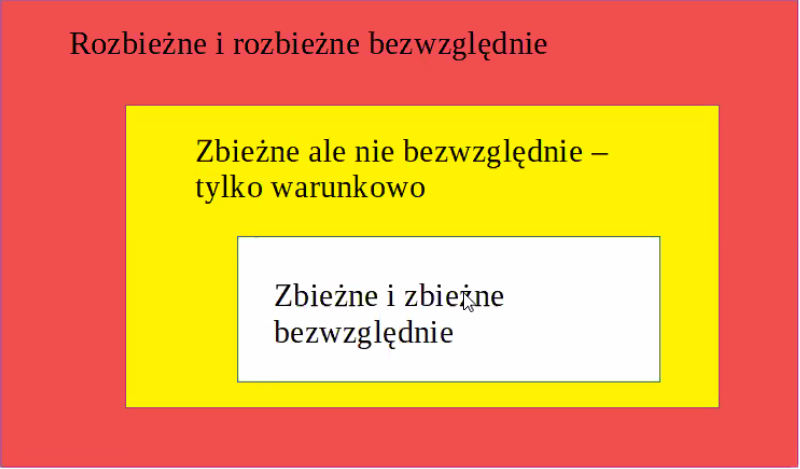
\includegraphics[scale=0.6]{rozbiezneirozbiezne.png}
\end{center}

Przykład 

Całka $ \int\limits_{1}^{\infty} \frac{\sin x}{\sqrt[3]{x^4}} \,dx $ jest zbieżna bezwględnie, bo biorąc
$ \int\limits_{1}^{\infty} \left| \frac{\sin x}{\sqrt[3]{x^4}} \right| \,dx $ i używając kryterium porównawczego mamy

$$ 0 \leq \left| \frac{\sin x}{\sqrt[3]{x^4}} \right| = \frac{|\sin x|}{x^{\frac{4}{3}}} \leq \frac{1}{x^{\frac{4}{3}}} $$

a całka $ \int\limits_{1}^{\infty} \frac{1}{x^{\frac{4}{3}}} \,dx $ jest zbieżna bo $ \frac{4}{3} > 1 $.
Zatem $ \int\limits_{1}^{\infty} \left| \frac{\sin x}{\sqrt[3]{x^4}} \right| \,dx $ jest zbieżna, a stąd
$ \int\limits_{1}^{\infty} \frac{\sin x}{\sqrt[3]{x^4}} \,dx $ też jest zbieżna.

\section{Szeregi liczbowe}

Dany jest ciąg liczbowy $ a_1, a_2, ..., a_n, ... $

Tworzymy jego ciąg sum częściowych :

$$ S_1 = a_1, \ \ S_2 = a_1 + a_2, \ \ S_n = a_1 + a_2 + ... + a_n = \sum\limits_{k = 1}^{n} a_k $$

Jeżeli istnieje granica $ S = \lim_{n \to \infty} S_n $ (skończona lub nieskończona) to oznaczamy ją symbolem 
$ \sum_{k = 1}^{\infty} a_k $. \\

W ogólnym przypadku możemy wziąć ciąg, który zaczyna się od dowolnej liczby całkowitej \linebreak $ n_0 $ : $ a_{n_0}, a_{n_0 + 1}, ..., a_n, ... $
i jego sum częściowych

$$ S_n = a_{n_0}, \ \ S_{n_0 + 1} = a_{n_0} + a_{n_0 + 1}, \ \ S_n = a_{n_0} + a_{n_0 + 1} + ... + a_n = \sum\limits_{k = n_0}^{n} a_k, \ n \geq n_0 $$

$ S = \lim_{n \to \infty} S_n $ jest oznaczana przez $ \sum\limits_{k = n_0}^{\infty} a_k $. \\

Definicja. Dla ustalonego $ n_0 \in \mathbb{Z} $ obiekt $ \sum\limits_{k = n_0}^{\infty} a_k $ nazywamy \underline{szeregiem liczbowym},
a wartość S (gdy istnieje) jego \underline{sumą}, oznaczaną także przez $ \sum\limits_{k = n_0}^{\infty} a_k $. Mamy wtedy

$$ S_n = a_{n_0}, \ \ S_{n_0 + 1} = a_{n_0} + a_{n_0 + 1}. \ \ S_n = a_{n_0} + a_{n_0 + 1} + ... + a_n + ... = 
\sum\limits_{k = n_0}^{\infty} a_k = \lim_{n \to \infty} \sum\limits_{k = n_0}^{n} a_k = \lim_{n \to \infty} S_n $$

gdzie

\begin{itemize}
    \item $ S_n $ to $n$ - ta suma szeregu,
    \item $ a_n $ to $n$ - ty wyraz szeregu. \\
\end{itemize}

Terminologia dotycząca sumy $S$ jest taka, jak dla ciągów. Są 3 przypadki : 

\begin{enumerate}
    \item $S$ jest liczbą. Wtedy dany szereg jest \underline{zbieżny} (do $S$).
    \item $S = \infty$ lub $S = -\infty$. Wtedy dany szereg jest \underline{rozbieżny} (do $\infty$ lub $-\infty$).
    \item $ S = \lim_{n \to \infty} S_n $ nie istnieje. Wtedy dany szereg jest \underline{rozbieżny}. \\
\end{enumerate}

Przykłady

$$ \frac{1}{2^1} + \frac{1}{2^2} + \frac{1}{2^3} + ... + \frac{1}{2^n} + ... = \sum\limits_{n = 1}^{\infty} \frac{1}{2^n} 
\textrm { - szereg zbieżny do 1}$$

$$ \frac{1}{2} + \frac{1}{3} + ... + \frac{1}{n} + ... = \sum\limits_{n = 2}^{\infty} \frac{1}{n} 
\textrm { - szereg rozbieżny do } \infty$$

$$ 1 - 1 + 1 - 1 + 1 - 1 + ... = \sum\limits_{n = 0}^{\infty} (-1)^n \textrm{ - szereg rozbieżny} $$

Uwaga. Każdy szereg zaczynający się od indeksu $ n_0 \in \mathbb{Z} $ można przekształcić tak, by zaczynał się od indeksu 1.
Wynika to z równości

$$ \sum\limits_{n = n_0}^{\infty} a_n = \sum\limits_{n = 1}^{\infty} a_{n + n_0 - 1} $$

$$ \frac{1}{2} + \frac{1}{3} + ... + \frac{1}{n} + ... = \sum\limits_{n = 2}^{\infty} \frac{1}{n} = \sum\limits_{n = 2}^{\infty} a_n
= \sum\limits_{n = 1}^{\infty} a_{n + 1} = \sum\limits_{n = 1}^{\infty} \frac{1}{n + 1} $$

\subsection*{Obliczanie sum szeregów}
\addcontentsline{toc}{subsection}{Obliczanie sum szeregów}

Jest to zadanie trudne, a najczęściej niemożliwe, gdyż trudno jest znaleźć bezpośredni wzór na sumy częściowe $S_n$. \\

Niektóre przypadki szczególne.

\begin{enumerate}
    \item Ciąg geometryczny i szereg geometryczny.
    \begin{itemize}
        \item 
        $ a_n = a_1 \cdot q^{n-1} $, gdzie $q$ jest ilorazem ciągu (czyli $a_{n+1} = a_n \cdot q , \ n \geq 1$).
        
        Wtedy

        $$ S_n = a_1 + a_2 + ... + a_n = a_1 \cdot \frac{1 - q^n}{1 - q}, q \neq 1 \ oraz \ S_n = na_1, \ q = 1 $$

        To oznacza, że dla $ a_1 \neq 0 $,

        \item szereg jest zbieżny dla $ -1 < q < 1 $ i jego suma jest $ S = \frac{a_1}{1 - q} $,
        \item szereg jest rozbieżny do $\infty$ lub $-\infty$ dla $ q \geq 1 $, znak zależy od znaku $a_1$,
        \item szereg jest rozbieżny (suma nie istnieje) dla $ q \leq -1 $ \\
    \end{itemize}

    Stąd np.

    $$ \frac{1}{2^1} + \frac{1}{2^2} + \frac{1}{2^3} + ... + \frac{1}{2^n} + ... = \sum\limits_{n = 1}^{\infty} \frac{1}{2^n} =
    \frac{ \frac{1}{2} }{ 1 - \frac{1}{2} } = 1 \ \textrm{, bo tutaj} \ a_1 = q = \frac{1}{2} $$

    \item Szeregi o wyrazie ogólnym postaci \\
    $ a_n = f(n + 1) - f(n)$ lub $ a_n = f(n) - f(n + 1) $, gdzie $f$ jest pewną funkcją.

    W bardziej ogólnej postaci \\
    \quad $ a_n = f(n + k) - f(n) $ lub $ a_n = f(n) - f(n + k) $, gdzie $ k \in \mathbb{N}^+ $ to tzw. krok. \\
    
    Takie szeregi to tzw. szeregi \underline{teleskopowe} (telescoping series).

    Przykłady

    $$ \sum\limits_{n = 1}^{\infty} \left( \frac{1}{n} - \frac{1}{n + 1} \right) \ \textrm{- tutaj} \ f(x) = \frac{1}{x} $$

    $$ \sum\limits_{n = 1}^{\infty} \left( \sqrt{n + 1} - \sqrt{n} \right) \ \textrm{- tutaj} \ f(x) = \sqrt{x} $$

    $$ \sum\limits_{n = 1}^{\infty} \left( \arctan(n) - \arctan(n+2) \right) \ \textrm{- tutaj} \ f(x) = \arctan x $$

    Dla takich szeregów łatwo wyznacza się wzór na $S_n$. Wyrazy wewnętrzne się upraszczają i zostaje: \\
    suma $k$ pierwszych wartości, \ $f$ suma $k$ ostatnich wartości $f$ (lub na odwrót) \\

\end{enumerate}

Na przykład dla $ \sum\limits_{n = 1}^{\infty} \left( f(n) - f(n + 1)) \right) $ mamy

$$ S_n = f(1) - \textcolor{red}{f(2)} + \textcolor{red}{f(2)} - \textcolor{blue}{f(3)} + \textcolor{blue}{f(3)} - 
\textcolor{green}{f(4)} + ... + \textcolor{purple}{f(n)} - f(n + 1) = f(1) - f(n + 1) $$.

Jeżeli istnieje granica $ G = \lim_{x \to \infty} f(x) $ to mamy

$$ S = \lim_{n \to \infty} S_n = \lim_{n \to \infty} \left( f(1) - f(n + 1) \right) = f(1) - G $$ \\

Przykład. Wyznaczyć sumę $ \sum\limits_{n = 1}^{\infty} \frac{1}{n^2 + n} $

Wyraz ogólny nie ma postaci różnicy więc trzeba ją stworzyć.

Używając rozkładu na ułamki proste dostajemy

$$ \frac{1}{n^2 + n} = \frac{1}{n(n+1)} = \frac{A}{n} + \frac{B}{n+1} = ... = \frac{1}{n} - \frac{1}{n+1} $$

Zatem 

$$ \sum\limits_{n = 1}^{\infty} \frac{1}{n^2 + n} = \sum\limits_{n=1}^{\infty} \left( \frac{1}{n} - \frac{1}{n+1} \right) $$

I to daje

$$ S_n = \left( \frac{1}{1} - \frac{1}{2} \right) + \left( \frac{1}{2} - \frac{1}{3} \right) + \left( \frac{1}{3} - \frac{1}{4} \right)
+ ... + \left( \frac{1}{n} - \frac{1}{n+1} \right) = \frac{1}{1} - \frac{1}{n+1}  $$ 

$$ \lim_{n \to \infty} S_n = 1 = \sum\limits_{n = 1}^{\infty} \frac{1}{n^2 + n} $$

\subsection*{Własności szeregów zbieżnych}
\addcontentsline{toc}{subsection}{Własności szeregów zbieżnych}

\textbf{Twierdzenie}

Jeżeli szeregi $ \sum\limits_{n = n_0}^{\infty} a_n $ oraz $ \sum\limits_{n = n_0}^{\infty} b_n $ są zbieżne to zbieżne są szeregi
$ \sum\limits_{n = n_0}^{\infty} (a_n + b_n) $ \linebreak oraz $ \sum\limits_{n = n_0}^{\infty} (c \cdot a_n), \ c \in \mathbb{R} $. \\

Ponadto

\begin{itemize}
    \item $ \sum\limits_{n = n_0}^{\infty} (a_n \pm b_n) = \sum\limits_{n = n_0}^{\infty} a_n \pm \sum\limits_{n = n_0}^{\infty} b_n $
    \item $ \sum\limits_{n = n_0}^{\infty} (c \cdot a_n) = c \sum\limits_{n = n_0}^{\infty} a_n $ \\
\end{itemize}

Prawdziwe są także analogiczne twierdzenia prowadzące do arytmetyki granic nieskończonych, gdy nie pojawiają się symbole nieoznaczone.
Na przykład gdy $ \sum\limits_{n = n_0}^{\infty} a_n = \infty $ oraz $ \sum\limits_{n = n_0}^{\infty} b_n = b \in \mathbb{R} $ to 

$$ \sum\limits_{n = n_0}^{\infty} (a_n \pm b_n) = \sum\limits_{n = n_0}^{\infty} a_n \pm \sum\limits_{n = n_0}^{\infty} b_n = \infty $$ \\

Natomiast gdy $ \sum\limits_{n = n_0}^{\infty} a_n = \sum\limits_{n = n_0}^{\infty} b_n = \infty $ to
$ \sum\limits_{n = n_0}^{\infty} (a_n - b_n) $ może być zarówno zbieżny jak i rozbieżny i nie ma sensu równość

$$ \sum\limits_{n = n_0}^{\infty} (a_n - b_n) = \sum\limits_{n = n_0}^{\infty} a_n - \sum\limits_{n = n_0}^{\infty} b_n $$ \\

\textbf{Twierdzenie}

Zmiana wartości $n_0$ nie wpływa na zbieżność/rozbieżność szeregu $ \sum\limits_{n = n_0}^{\infty} a_n $.

Może mieć wpływ na wartość jego sumy. \\

Stąd wynika np., że szeregi $ \sum\limits_{n = 1}^{\infty} a_n $ i $ \sum\limits_{n = 100}^{\infty} a_n $ są albo oba zbieżne
albo oba rozbieżne do $ \infty $ lub $-\infty$ albo oba rozbieżne.

To też oznacza, że na podstawie kilku pierwszych wyrazów ciągu/szeregu

\colorbox{yellow}{NIC NIE MOŻNA POWIEDZIEĆ} o jego zbieżności \\

\colorbox{red}{Popularny błąd}

"Liczymy wartości $ a_1, a_2, a_3, a_4, a_5$ . Wychodzi ciąg malejący i dodatni.

\textcolor{red}{Zatem szereg jest zbieżny}". \textbf{GAME OVER...} \\

\textbf{Twierdzenie}

Dla ustalonego $ n_0 \in \mathbb{N}^+ $ i $ p \in \mathbb{R} $ szereg $ \sum\limits_{n = n_0}^{\infty} \frac{1}{n^p} $
jest zbieżny dla $ p > 1 $ i rozbieżny do $\infty$ dla $p \leq 1$.  \\

W przypadku kiedy sumy szeregu nie da się wyznaczyć w sposób dokładny można to zrobić w sposób przybliżony, pod warunkiem, że wiemy,
że szereg jest zbiezny. \\

Kryteria zbieżności to twierdzenia opisujące warunki dostateczne zbieżności lub rozbieżności danej klasy szeregów. Najczęściej mają postać
implikacji ale \textbf{NIE} równoważności. \\

Oznacza to zwykle własności postaci

\quad warunek zachodzi $ \Rightarrow $ szereg jest zbieżny/rozbieżny,

\quad warunek nie zachodzi $\Rightarrow$ nic nie wiemy o zbieżności/rozbieżności szeregu \\

\subsection*{Popularne kryteria zbieżności szeregów}
\addcontentsline{toc}{subsection}{Popularne kryteria zbieżności szeregów}

0. Warunek konieczny zbieżności szeregów \\ 

\textbf{Twierdzenie}

Jeżeli szereg $ \sum\limits_{n = n_0}^{\infty} a_n $ jest zbieżny to $ \lim_{n \to \infty} a_n = 0 $. \\

Dowód 

Dla $ n \geq n_0 + 1 $ mamy $ S_n = a_{n_0} + a_{n_0 + 1} + ... + a_{n - 1} + a_n $ oraz 
$ S_{n - 1} = a_{n_0} + a_{n_0 + 1} + ... + a_{n - 1} $,

Stąd

$$ S_n - S_{n - 1} = a_n $$ \\

Jeżeli szereg $ \sum\limits_{n = n_0}^{\infty} a_n $ jest zbieżny to $ \lim_{n \to \infty} S_n = \lim_{n \to \infty} S_{n - 1} = S \in \mathbb{R} $.
To daje

$$ \lim_{n \to \infty} a_n = \lim_{n \to \infty} (S_n - S_{n - 1}) = \lim_{n \to \infty} S_n - \lim_{n \to \infty} S_{n - 1} = S - S = 0 $$ \\

Transpozycja tego twierdzenia daje warunek równoważny do zastosowania praktycznego :

Jeżeli $ \lim_{n \to \infty} a_n \neq 0 $ to szereg $ \sum\limits_{n = n_0}^{\infty} a_n $ nie jest zbiezny przy czym

\begin{itemize}
    \item gdy $ \lim_{n \to \infty} a_n > 0 $ to $ \sum\limits_{n = n_0}^{\infty} a_n = \infty $
    \item gdy $ \lim_{n \to \infty} a_n < 0 $ to $ \sum\limits_{n = n_0}^{\infty} a_n = -\infty $ 
\end{itemize}

\colorbox{yellow}{Uwaga. To jest tylko implikacja!}

Jeżeli $ \lim_{n \to \infty} a_n = 0 $ to jeszcze \colorbox{yellow}{NIC NIE WIEMY} o szeregu.

Na przykład szeregi $ \sum\limits_{n = n_0}^{\infty} \frac{1}{n^p} $ mają $ \lim_{n \to \infty} \frac{1}{n^p} = 0 $
dla wszystkich $ p > 0 $ ale niektóre z tych szeregów są zbieżne, a niektóre rozbieżne. \\

\colorbox{red}{Popularny błąd}

"$\lim_{n \to \infty} a_n = 0 $ \textcolor{red}{zatem szereg jest zbieżny}". \textbf{GAME OVER...} \\

Szeregi o wyrazach nieujemnych

$$ \sum\limits_{n = n_0}^{\infty} a_n, \ a_n \geq 0 $$

Wtedy $ S_n = a_{n_0} + a_{n_0 + 1} + ... + a_{n - 1} + a_n $ jest ciągiem niemalejącym zatem suma szeregu
$ \sum\limits_{n = n_0}^{\infty} a_n = \lim_{n \to \infty} S_n $ zawsze istnieje. Może być to liczba lub $\infty$.

Podobnie dla szeregów o wyrazach niedodatnich $ \sum\limits_{n = n_0}^{\infty} a_n, \ a_n \leq 0 $, suma zawsze istnieje
i rozbieżność oznacza rozbieżność do $-\infty$. \\

Przykład. Następujące szeregi nie są zbieżne

$$ \sum\limits_{n = 1}^{\infty} 1, \ \ \sum\limits_{n = 1}^{\infty} (n^2 + 2n), \ \
\sum\limits_{n = 1}^{\infty} \frac{n+1}{n+2}, \ \ \sum\limits_{n = 1}^{\infty} \left(1 + \frac{1}{n} \right)^n , \ \ 
\sum\limits_{n = 1}^{\infty} (-1)^n , \ \ \sum\limits_{n = 1}^{\infty} \sin n$$

Dla szeregów o wyrazach nieujemnych mamy dwa kolejne kryteria zbieżności.

\begin{enumerate}
    \item Kryterium porównawcze
    \item Kryterium ilorazowe \\
\end{enumerate} 

\subsection*{Twierdzenie (kryterium porównawcze)}
\addcontentsline{toc}{subsection}{Twierdzenie (kryterium porównawcze)}

Dane są dwa szeregi $ \sum\limits_{n = n_0}^{\infty} a_n $ oraz $ \sum\limits_{n = n_0}^{\infty} b_n $. Wtedy zachodzą nastepujące
własności.

\begin{enumerate}
    \item (Przypadek zbieżności) Gdy $ \forall n \geq k \geq n_0 \quad 0 \leq a_n \leq b_n $ i $ \sum\limits_{n = n_0}^{\infty} b_n $
    jest zbieżny to $ \sum\limits_{n = n_0}^{\infty} a_n $ też jest zbieżny. Ponadto
    $ 0 \leq \sum\limits_{n = n_0}^{\infty} a_n \leq \sum\limits_{n = n_0}^{\infty} b_n $
    
    \item (Przypadek rozbieżności) Gdy $ \forall n \geq k \geq n_0 \quad 0 \leq b_n \leq a_n $ i $ \sum\limits_{n = n_0}^{\infty} b_n $
    jest rozbieżny to $ \sum\limits_{n = n_0}^{\infty} a_n $ też jest rozbieżny. Ponadto
    $ \sum\limits_{n = n_0}^{\infty} a_n = \sum\limits_{n = n_0}^{\infty} b_n = \infty $

    \item (Przypadek wątpliwy). Gdy $ \forall n \geq k \geq n_0 \quad 0 \leq a_n \leq b_n $ ale $ \sum\limits_{n = n_0}^{\infty} b_n $ jest
    rozbieżny to \textbf{NIC NIE WIEMY} o zbieżności $ \sum\limits_{n = n_0}^{\infty} a_n $

    \item (Przypadek wątpliwy). Gdy $ \forall n \geq k \geq n_0 \quad 0 \leq b_n \leq a_n $ ale $ \sum\limits_{n = n_0}^{\infty} b_n $ jest
    zbieżny to \textbf{NIC NIE WIEMY} o zbieżności $ \sum\limits_{n = n_0}^{\infty} a_n $ \\
\end{enumerate}

Uwagi

\begin{itemize}
    \item $ \sum\limits_{n = n_0}^{\infty} a_n $ jest szeregiem z zadania, $ \sum\limits_{n = n_0}^{\infty} b_n $ tworzymy sami
    \item Porównujemy najczęściej z szeregiem geometrycznym $ \sum\limits_{n = n_0}^{\infty} q^n $ lub z szeregami
    $ \sum\limits_{n = n_0}^{\infty} \frac{1}{n^p} $. Wtedy $a_n$ często ma postać ułamków i możemy spróbować wziąć $b_n$ jako

    \quad \colorbox{yellow}{C $\cdot$ iloraz najwyższych potęg z licznika i mianownika $a_n$} 

    \item Trzeba uważać aby nierówność między $a_n$ i $b_n$ była prawdziwa i nie zapomnieć o dolnym ograniczeniu (0). Ma być
    tak jak w \underline{twierdzeniu o trzech ciągach}

    \item Kryterium nie zawsze jest wygodne w użyciu i trzeba uważać, by nie dostać przypadku wątpliwego, bo wtedy \textbf{trzeba zaczynać od nowa}
    
    \item Warto sprawdzić opisany wyżej iloraz najwyższych potęg i na tej podstawie przewidzieć czy chcemy udowodnić zbieżność
    czy rozbieżność. To pomaga skonstruować odpowiednią nierówność między $a_n$ i $b_n$.
\end{itemize}

\colorbox{red}{Popularny błąd : } odpowiedź na podstawie przypadku wątpliwego

Na przykład dla szeregu $ \sum\limits_{n = 1}^{\infty} \frac{1}{n + \sqrt{n}} : $

"Mamy $ 0 \leq \frac{1}{n + \sqrt{n}} \leq \frac{1}{n} $ i szereg $ \sum\limits_{n = 1}^{\infty} \frac{1}{n} $
jest rozbieżny \textcolor{red}{zatem szereg $\sum\limits_{n = 1}^{\infty} \frac{1}{n + \sqrt{n}}$ jest rozbieżny}". \\

\textbf{GAME OVER...} To jest przypadek nr 3 (wątpliwy) \\

Przykład

$$ \sum\limits_{n = 4}^{\infty} \frac{2n - 3}{n^3 - 1} $$

Przewidywanie zbieżności/rozbieżności:

Iloraz najwyższych potęg licznika i mianownika to $ \frac{n}{n^3} = \frac{1}{n^2} $, a szereg $ \sum\limits_{n = 4}^{\infty} \frac{1}{n^2} $
jest zbieżny, bo $ 2 > 1 $. Zatem chcemy udowodnić zbieżność (przypadek 1).

Potrzebujemy więc $ \sum\limits_{n = 4}^{\infty} b_n $ i nierówności $ 0 \leq \frac{2n - 3}{n^3 - 1} \leq b_n $.

Chcemy zwiększyć wyrażenie $ \frac{2n - 3}{n^3 - 1} $ ale tak, by \colorbox{yellow}{zostały najwyższe potęgi}.

Można zwiększyć \underline{licznik} oraz \underline{zmniejszyć mianownik}.

Zwiększamy licznik poprzez wyrzucenie 3.

Zmniejszamy mianownik poprzez zastąpienie 1 czymś większym : wyrażeniem z najwyższą potęgą. Nie można jednak wziąć całego $n^3$
, bo będzie 0 w mianowniku.

Wygrywa wzięcie $ C \cdot n^3 $ np. $ \frac{1}{2} n^3 $, bo dla $ n \geq 4 $ mamy $ \frac{1}{2} n^3 \geq 1 $.

To wszystko daje dla $ n \geq 4 $

$$ 0 \leq \frac{2n - 3}{n^3 - 1} \leq \frac{2n}{n^3 - \frac{1}{2} n^3} $$

Czyli

$$ b_n = \frac{2n}{n^3 - \frac{1}{2}n^3} = 4 \cdot \frac{1}{n^2} $$

\textbf{DZIURA W SKRYPCIE}

\subsection*{Twierdzenie (kryterium ilorazowe)}
\addcontentsline{toc}{subsection}{Twierdzenie (kryterium ilorazowe)}

Dane są dwa szeregi $ \sum\limits_{n = n_0}^{\infty} a_n $ oraz $ \sum\limits_{n = n_0}^{\infty} b_n $.
Ponadto $ \forall n \geq n_0 \ a_n, b_n > 0 $.

Jeżeli istnieje granica $ \lim_{n \to \infty} \frac{a_n}{b_n} $ i jest \colorbox{yellow}{liczbą dodatnią} to wtedy oba
szeregi są zbieżne albo oba rozbieżne do $\infty$. \\

Uwagi

\begin{itemize}
    \item Ciąg $b_n$ tworzymy podobnie jak dla kryterium porównawczego.
    \item Nie ma problemu z nierównościami :) ale za to trzeba umiećl liczyć granice.
    \item Granica nie może być ani 0 ani $\infty$: \ $ \lim_{n \to \infty} \frac{a_n}{b_n} = L \in (0, \infty) $.
    
    \colorbox{yellow}{Nie wystarczy warunek $L > 0$ bo $\infty$ także jest $ > 0$.}
    \item Rozwiązanie \colorbox{yellow}{musi zawierać wniosek} "granica ilorazu jest liczbą dodatnią więc oba
    \colorbox{yellow}{szeregi} są zbieżne lub oba rozbieżne" - bez tego będzie niepełne
    
    \item Kryterium zwykle jest wygodniejsze niż porównawcze ale są przykłady, które pójdą z porównawczego ale nie z
    ilorazowego, bo granica ilorazu nie istnieje
    
    Np. \ $ \sum\limits_{n = 1}^{\infty} \frac{2 + \sin n}{n} $.
\end{itemize}

Przykłady

Poprzedni przykład raz jeszcze 

$$ \sum\limits_{n = 4}^{\infty} \frac{2n - 3}{n^3 - 1} $$

Bierzemy $ b_n = \frac{n}{n^3} = \frac{1}{n^2} $

$$ \dfrac{a_n}{b_n} = \dfrac{\dfrac{2n - 3}{n^3 - 1}}{\dfrac{1}{n^2}} = \dfrac{2n^3 - 3n^2}{n^3 - 1}
= \dfrac{2 - \dfrac{3}{n}}{1 - \dfrac{1}{n^3}} $$ \\

Stąd $ \lim_{n \to \infty} \frac{a_n}{b_n} = 2 $ - liczba dodatnia.

Zatem oba szeregi są zbieżne lub oba są rozbieżne.

Dalej już analiza $ \sum\limits_{n = 4}^{\infty} \frac{1}{n^2} $ i wniosek jak w kryterium porównawczym :

$ \sum\limits_{n = 4}^{\infty} b_n = \sum\limits_{n = 4}^{\infty} \frac{1}{n^2} $ jest zbieżny bo $ 2 > 1 $.
Zatem $ \sum\limits_{n = 4}^{\infty} \frac{2n - 3}{n^3 - 1} $ też jest zbieżny. \\\\

Przykłady o postaci funkcji złożonej $ \sum\limits_{n = n_0}^{\infty} f(b_n) $,

gdzie $ \lim_{n \to \infty} b_n = 0^+ $ oraz $ \lim_{x \to 0^+} f(x) = 0^+ $.

Nowym szeregiem jest szereg z funkcji wewnętrznej $ \sum\limits_{n = n_0}^{\infty} b_n $.

Liczymy granicę 

$$ \lim_{n \to \infty} \frac{f(b_n)}{b_n} = \lim_{x=b \to 0^+} \frac{f(x)}{x} \left[ \frac{0}{0} \right] $$

przy użyciu granic podstawowych lub reguły de l'Hospitala. \\

Na przykład

$$ \sum\limits_{n = 1}^{\infty} \left( \sqrt[n]{2} - 1 \right) $$

Mamy $$ \sum\limits_{n = 1}^{\infty} \left( \sqrt[n]{2} - 1 \right) = \sum\limits_{n = 1}^{\infty} \left( 2^{\frac{1}{n}} - 1 \right) $$

Więc bierzemy $ b_n = \frac{1}{n} > 0 $.

Liczymy granicę

$$ \lim_{n \to \infty} \frac{2^{\frac{1}{n}} - 1}{\frac{1}{n}} = \lim_{x = \frac{1}{n} \to 0^+} \frac{2^x - 1}{x} = \ln 2 $$ \\

Jest to liczba dodatnia więc oba szeregi są zbieżne lub oba są rozbieżne.

$ \sum\limits_{n = 1}^{\infty} \frac{1}{n} = \infty $ więc $ \sum\limits_{n = 1}^{\infty} \left( \sqrt[n]{2} - 1 \right) = \infty $. \\ \\

3. Kryterium Cauchy'ego.

4. Kryterium d'Alemberta \\

Działają dla szeregów o dowolnych wyrazach. Teza obu kryteriów jest taka sama ale liczymy granice innych wyrażeń.


\subsection*{Twierdzenie (kryterium Cauchy'ego)}
\addcontentsline{toc}{subsection}{Twierdzenie (kryterium Cauchy'ego)}

Dany jest szereg $ \sum\limits_{n = n_0}^{\infty} a_n $ taki, że istnieje granica $ q = \lim_{n \to \infty} \sqrt[n]{|a_n|} $. Wtedy

\begin{enumerate}
    \item Gdy $ 0 \leq q < 1 $ to szereg jest zbieżny.
    \item Gdy $ q > 1 $ to szereg jest rozbieżny
    \item \textbf{(Przypadek wątpliwy)}. Gdy q = 1 to \colorbox{yellow}{NIC NIE WIEMY} o zbieżności szeregu. \\
\end{enumerate}

\textbf{Uwagi}

\begin{itemize}
    \item Do wyznaczenia $q$ przydają się następujące właśności granic
    
    a) Gdy $ \lim_{n \to \infty} a_n $ jest \textbf{liczbą dodatnią} to $ \lim_{n \to \infty} \sqrt[n]{a_n} = 1 $.

    b) $ \forall p \in \mathbb{R} \ \lim_{n \to \infty} \sqrt[n]{n^p} = 1 $.

    \item \textbf{$q$ nie może być ujemne}. $q$ ujemne zwykle oznacza brak modułu na $a_n$.
\end{itemize}


\subsection*{Twierdzenie (kryterium d'Alemberta)}
\addcontentsline{toc}{subsection}{Twierdzenie (kryterium d'Alemberta)}

Dany jest szereg $ \sum\limits_{n = n_0}^{\infty} a_n, \ a_n \neq 0 $, taki, że istnieje granica
$ q = \lim_{n \to \infty} \left| \frac{a_{n + 1}}{a_n} \right| $. Wtedy

\begin{enumerate}
    \item Gdy $ 0 \leq q < 1 $ to szereg jest zbieżny.
    \item Gdy $ q > 1 $ to szereg jest rozbieżny
    \item \textbf{(Przypadek wątpliwy)}. Gdy q = 1 to \colorbox{yellow}{NIC NIE WIEMY} o zbieżności szeregu. \\
\end{enumerate}

\begin{itemize}
    \item \textbf{$q$ nie może być ujemne}. $q$ ujemne zwykle oznacza brak modułu na $a_n$.
    
    \item W obu kryteriach szerergi $ \sum\limits_{n = n_0}^{\infty} \frac{1}{n^p} $ pokazują, że $ q = 1$ nic nie daje. \\
\end{itemize}

Przykłady

$$ \sum\limits_{n = 1}^{\infty} \frac{20^n}{n!} $$

Tutaj $ a_n = \frac{20^n}{n!} > 0 $ oraz $ a_{n + 1} = \frac{20^{n + 1}}{(n + 1)!} $. Zatem z kryterium d'Alemberta

$$ q = \lim_{n \to \infty} \left| \frac{a_{n + 1}}{a_n} \right| = \frac{ \dfrac{20^{n + 1}}{(n+1)!} }{ \dfrac{20^n}{n!} } $$ \\

$$ \sum\limits_{n = 1}^{\infty} \left( 2\arcsin \frac{1 - n}{2n + 1} \right)^n $$

Tutaj chcemy użyć kryterium Cauchy'ego.

$$ \sqrt[n]{|a_n|} = \sqrt[n]{ \left| \left( 2\arcsin \frac{1-n}{2n+1} \right)^n \right| } 
= \sqrt[n]{ \left| 2\arcsin \frac{1-n}{2n+1} \right|^n } = \left| 2\arcsin \frac{1-n}{2n+1} \right|
= \left| 2\arcsin \frac{ \dfrac{1}{n} - 1  }{ 2 + \dfrac{1}{n} } \right| $$

Stąd 

$$ q = \lim_{n \to \infty} \sqrt[n]{|a_n|} = \left| 2\arcsin \left( -\frac{1}{2} \right) \right|
= \left| 2 \left( - \frac{\pi}{6} \right) \right| = \frac{\pi}{3} $$

$q > 1$ więc szereg jest rozbieżny.


\subsection*{Twierdzenie (kryterium całkowe)}
\addcontentsline{toc}{subsection}{Twierdzenie (kryterium całkowe)}

Dany jest szereg $ \sum\limits_{n = n_0}^{\infty} a_n $. Jeżeli na $ [x_0, \infty), \ x_0 \geq n_0 $ istnieje funkcja $f$
taka, że 

\begin{itemize}
    \item $ f(n) = a_n, \ n \geq x_0 $,\
    \item $f$ jest nieujemna na $[x_0, \infty)$,
    \item $f$ jest nierosnąca na $[x_0, \infty)$,
\end{itemize}

to całka niewłaściwa $ \int\limits_{x_0}^{\infty} f(x) \,dx $ i szereg $ \sum\limits_{n = n_0}^{\infty} a_n $ są
jednocześnie skończone lub jednocześnie rozbieżne do $\infty$. \\

Uwagi do kryterium

\begin{itemize}
    \item Najczęściej $ x_0 = n_0 $.
    \item Kryterium jest ważne z punktu widzenia teorii, gdyż wiele innych własności szeregów z niego wynika.
    Na przykład, gdy $x_0 = n_0$ to
    $$ \int\limits_{n_0}^{\infty} f(x) \,dx \leq \sum\limits_{n = n_0}^{\infty} a_n \leq 
    a_{n_0} + \int\limits_{n_0}^{\infty} f(x) \,dx $$
    To pozwala oszacować sumę szeregu.

    \item Sens użycia kryterium: nie umiemy policzyć sumy szeregu ale umiemy \textbf{obliczyć} całkę
    $ \int\limits_{x_0}^{\infty} f(x) \,dx = \lim_{T \to \infty} \int\limits_{x_0}^{T} f(x) \,dx $. Stosujemy to
    kryterium tylko wtedy, gdy zamierzamy liczyć tę całkę.

    \item Z praktycznego punktu widzenia kryterium jest najczęściej \colorbox{yellow}{najmniej wygodnie} do zastosowania.
    Opłaca się je stosować głównie wtedy, gdy szereg zawiera wyrażenie $\ln n$. \\
\end{itemize}

Przykład

Dla ustalonego $ n_0 \in \mathbb{N}^+ $ i $p > 0$ dowodzimy znany już wynik dla szeregu $ \sum\limits_{n = n_0}^{\infty} \frac{1}{n^p} $
zbieżny dla $p > 1$ oraz rozbieżny do $\infty$ dla $p \leq 1$. \\

Tutaj bierzemy po prostu $ f(x) = \frac{1}{x^p}, \ x \in [n_0, \infty) $.

Dla $p > 0$ $f$ jest malejąca i nieujemna oraz $ f(n) = \frac{1}{n^p} $ 

Spełnione są wiec warunki użycia kryterium. Liczymy całkę $ \int\limits_{n_0}^{\infty} \frac{1}{x^p} \,dx $.

Było to już robione wcześniej i wiemy, że dla $p > 1$ jest liczbą, a dla $p \leq 1$ jest równa $\infty$.
Stąd szereg jest zbieżny dla $p > 1$ oraz rozbieżny do $\infty$ dla $0 < p \leq 1$. Dla $p \leq 0$ szereg jest rozbieżny,
bo nie spełnia warunku koniecznego zbieżności. \\

Uwaga do szeregów z wyrażeniem $\ln n$.

Dla dowolnego $p>0$ funkcja $\frac{\ln x}{x^p}, \ x \geq 2$, ma zbiór wartości $\left( 0, \frac{1}{p \cdot e} \right]$. Zatem

$$ \frac{\ln x}{x^p} \leq \frac{1}{p \cdot e} \Leftrightarrow \ln x \leq \frac{1}{p \cdot e} x^p $$

a stąd

$$ \ln n \leq \frac{1}{p \cdot e} n^p $$

Z oszacowaniem dolnym jest gorzej, bo nie ma pojedynczej funkcji elementarnej mniejszej od $\ln x$ i pozostaje oszacowanie
przez stałą np.

$$ \ln n \geq \frac{1}{2}, \quad n \geq 2  $$

To daje oszacowanie dla dowolnego $p>0$:

$$ \frac{1}{2} \leq \ln n \leq C \cdot n^p, \quad n \geq 2 $$

Tutaj $ C = \frac{1}{p \cdot e} $, a dla $ p \geq \frac{1}{e} $ wystarczy wziąć $C = 1$.

Często to oszacowanie pozwala uniknąć kryterium całkowego i zastąpienie go porównawczym, potrzeba tylko wziąć
odpowiednio małe p. \\

Przykład

Dla szeregu $ \sum\limits_{n = 2}^{\infty} \frac{\ln n}{n \sqrt[5]{n}} $ z kryterium porównawczego mamy

$$ 0 < \frac{\ln n}{n \sqrt[5]{n}} \leq \frac{Cn^p}{n \sqrt[5]{n}} = \frac{Cn^p}{n \cdot n^{0,2}} = \frac{C}{n^{1,2 - p}} $$

Wystarczy teraz wziąć $p < 0,2$ czyli np. $p = 0,1$ i zbadać szereg

$$ \sum\limits_{n=2}^{\infty} \frac{C}{n^{1,2 - 0,1}} = C \sum\limits_{n=2}^{\infty} \frac{C}{n^{1,1}} 
\ \ \textrm{--- zbieżny, bo} \ 1,1 > 1$$

Zatem wyjściowy szereg jest zbieżny


\subsection*{Zbieżność bezwględna szeregów}
\addcontentsline{toc}{subsection}{Zbieżność bezwględna szeregów}

Definicja. Szereg $ \sum\limits_{n=n_0}^{\infty} a_n$ jest \underline{zbieżny bezwględnie}, gdy zbieżny jest szereg
$ \sum\limits_{n=n_0}^{\infty} |a_n|$. \\

Uwagi

\begin{itemize}
    \item Gdy wszystkie wyrazy $a_n$ są nieujemne to mamy $\sum\limits_{n=n_0}^{\infty} a_n = \sum\limits_{n=n_0}^{\infty} |a_n|$
    i definicja nie wnosi nic nowego. Sytuacja się zmienia gdy szereg ma zarówno wyrazy dodatnie jak i ujemne.
    \item Z nierówności $|S_n|= |a_{n_0} + a_{n_0+1} + ... + a_n| \leq |a_{n_0}| + |a_{n_0 + 1}| + ... + |a_n| $
    wynika nierówność $ \left| \sum\limits_{n=n_0}^{\infty} a_n \right| \leq \sum\limits_{n=n_0}^{\infty} |a_n| $
    ale równość nie musi zachodzić.

    Np. dla $ a_n = \left( -\frac{1}{2} \right)^n $ mamy $ \left| \sum\limits_{n=0}^{\infty} a_n \right| = \frac{2}{3} $
    \ ale \ $  \sum\limits_{n=0}^{\infty} |a_n| = 2 $

    Zatem $ \left| \sum\limits_{n=n_0}^{\infty} a_n \right| $ \ i \ $ \sum\limits_{n=n_0}^{\infty} |a_n| $ \textbf{to nie to samo}. \\
\end{itemize}

\textbf{Twierdzenie}

Jeżeli szereg jest bezwględnie zbieżny to jest zbieżny (w zwykłym sensie).

Transpozycja tego twierdzenia daje warunek równoważny:

Jeżeli szereg $ \sum\limits_{n = n_0}^{\infty} a_n $ nie jest zbieżny to również nie jest zbieżny bezwględnie, co oznacza
$ \sum\limits_{n=n_0}^{\infty} |a_n| = \infty $.

Twierdzenie odwrotne nie jest prawdziwe. Są szeregi zbieżne ale nie bezwględnie, np.
$ \sum\limits_{n=1}^{\infty} \frac{(-1)^n}{n} $. Takie szeregi to tzw. szeregi \underline{zbieżne warunkowo}. \\

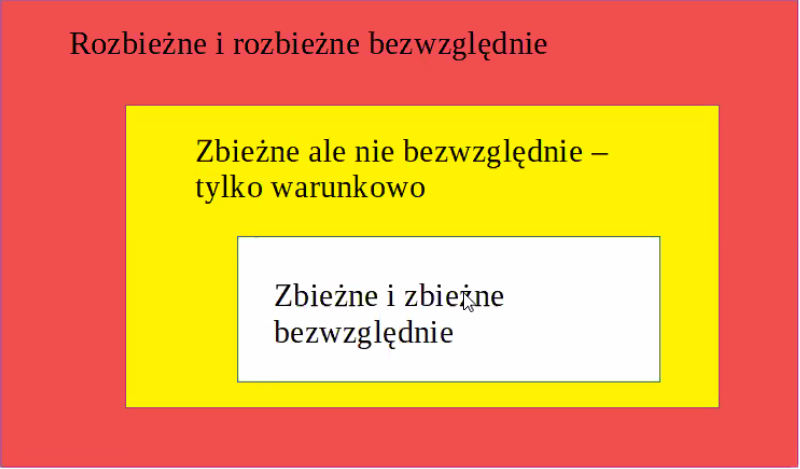
\includegraphics[scale=0.6]{rozbiezneirozbiezne.png} \\

Przykład 

Szereg $ \sum\limits_{n=1}^{\infty} \frac{\sin n}{\sqrt[3]{n^4}} $ jest zbieżny bezwględnie, bo biorąc
$ \sum\limits_{n=1}^{\infty} \left| \frac{\sin n}{\sqrt[3]{n^4}} \right| $ i używając kryterium porównwawczego mamy

$$ 0 \leq \left| \frac{\sin n}{\sqrt[3]{n^4}} \right| = \frac{|\sin n|}{n^{\frac{4}{3}}} \leq \frac{1}{n^{\frac{4}{3}}} $$

a szereg $ \sum\limits_{n=1}^{\infty} \frac{1}{n^{\frac{4}{3}}} $ jest zbieżny, bo $ \frac{4}{3} > 1 $. 

Zatem
$ \sum\limits_{n=1}^{\infty} \left| \frac{\sin n}{\sqrt[3]{n^4}} \right| $, a stąd
$\sum\limits_{n=1}^{\infty} \frac{\sin n}{\sqrt[3]{n^4}}$ też jest zbieżny.


\subsection*{Szeregi naprzemienne}
\addcontentsline{toc}{subsection}{Szeregi naprzemienne}

Są to szeregi, w których na zmianę dodajemy i odejmujemy wyrazy dodatnie:

$ a_{n_0} - a_{n_0 + 1} + a_{n_0 + 2} - a_{n_0 + 3} + ... $ \ lub \ $ -a_{n_0} + a_{n_0 + 1} - a_{n_0 + 2} + a_{n_0 + 3} + ...  $ \
gdzie $a_n > 0$. \\

Postać ogólna :

$ \sum\limits_{n = n_0}^{\infty} (-1)^n \cdot a_n $ \ lub \ $ \sum\limits_{n = n_0}^{\infty} (-1)^{n+1} \cdot a_n $ \\

Przykłady

$$ \sqrt{2} - \sqrt{3} + \sqrt{4} - \sqrt{5} + ... = \sum\limits_{n=2}^{\infty} (-1)^n \sqrt{n} $$

$$ 1 - \frac{1}{2} + \frac{1}{3} - \frac{1}{4} + ... = \sum\limits_{n=1}^{\infty} \frac{(-1)^{n+1}}{n} $$ \\

Definicja

Szereg naprzemienny $ \sum\limits_{n = n_0}^{\infty} (-1)^n \cdot a_n $ \ lub \ $ \sum\limits_{n = n_0}^{\infty} (-1)^{n+1} \cdot a_n $
nazywany jest \underline{szeregiem Leibnitza}, jeżeli $a_n$ jest ciągiem nierosnącym i zbieżnym do 0.

Na przykład $ 1 - \frac{1}{2} + \frac{1}{3} - \frac{1}{4} + ... = \sum\limits_{n=1}^{\infty} \frac{(-1)^{n+1}}{n} $
jest szeregiem Leibnitza, bo tutaj $ a_n = \frac{1}{n} $ jest malejący i zbieżny do 0. \\

\textbf{Twierdzenie (Leibnitz)}

Każdy szereg Leibnitza jest zbieżny. \\

Uwagi

\begin{itemize}
    \item Tiwerdzenie to daje tylko zbieżność warunkową, nie gwarantuje bezwględnej
    \item Gdy ciąg $a_n$ nie dąży do 0 to szereg naprzemienny $ \sum\limits_{n = n_0}^{\infty} (-1)^n \cdot a_n $ jest
    rozbieżny, gdyż $(-1)^n a_n$ też nie dąży do 0. Wynika to z twierdzenia

    $$ \lim_{n \to \infty} a_n = 0 \Leftrightarrow \lim_{n \to \infty} (-1)^n a_n = 0 \Leftrightarrow \lim_{n \to \infty} |a_n| = 0$$

    \item Wystarczy, by ciąg $a_n$ był nierosnący dla $ \forall n \geq k \geq n_0$.
    \item Gdy ciąg $a_n$ zbiega do 0 ale nie jest nierosnący to \textbf{NIC NIE WIEMY} o zbieżności szeregu.
    \item Do badania czy $a_n$ jest nierosnący można próbować rozszerzyć $a_n$ do funkcji $f$ tak by $f(n) = a_n$.
    Potem --- pochodna itd.
    Gdy szereg naprzemienny jest zbieżny bezwględnie to tw. Leibnitza nie jest potrzebne. \\
\end{itemize}

\textbf{Popularny błąd : } opisowanie "badanie" monotoniczności ciągu, bez obliczeń.

Na przykład dla ciągu $ a_n = \frac{n}{1000n + 1} $ :

"Ciąg $a_n$ jest \textcolor{red}{malejący}, bo mianownik \textcolor{red}{szybciej rośnie niż licznik}."

GAME OVER... \ Takie "rozwiązanie" jest jak \colorbox{yellow}{pisanie bajek} --- nie musi mieć \linebreak
\colorbox{yellow}{nic wspólnego z prawdą}.

Dla powyższego ciągu mianownik rzeczywiście szybciej rośnie niż licznik (i to 1000 razy!), a mimo to ciąg ten jest rosnący. \\

Przykład

$$ \sum\limits_{n=2}^{\infty} \frac{(-1)^n \cdot \ln n}{n} $$

Tutaj $ a_n = \frac{\ln n}{n} $. Rozszerzamy go do funkcji $ f(x) = \frac{\ln x}{x}, \ x \geq 2 $.

$$ f'(x) = \frac{1 - \ln x}{x^2} < 0 \Leftrightarrow x > e \approx 2,72 $$

Zatem $f$ jest malejąca dla $ x \in (e, \infty) $ czyli $a_n$ jest malejący dla $n \geq 3$.

Ponadto

$$ \lim_{x \to \infty} f(x) = \lim_{x \to \infty} \frac{\ln x}{x} = \left[ \frac{\infty}{\infty} \right][H]
= \lim_{x \to \infty} \frac{\frac{1}{x}}{1} = 0 $$

Zatem $ \lim_{n \to \infty} a_n = 0 $.

Mamy więc szereg naprzemienny, który z tw. Leibnitza jest zbieżny.

Nie jest jednak zbieżny bezwględnie bo dla $ \sum\limits_{n=2}^{\infty} \left| \frac{(-1)^n \cdot \ln n}{n} \right|
= \sum\limits_{n=2}^{\infty} \frac{\ln n}{n} $ mamy z kryterium porównawczego $0 < \frac{0,5}{n} < \frac{\ln n}{n}$,
a szereg $ \sum\limits_{n=2}^{\infty} \frac{0,5}{n} $ jest rozbieżny.

Jest to więc szereg zbieżny warunkowo. \\

Podsumowanie : które kryterium zbieżności kiedy?

\begin{itemize}
    \item P --- porównawcze
    \item I --- ilorazowe
    \item C - Cauchy'ego
    \item A - d'Alemberta
    \item $\int$ --- całkowe
    \item ZB --- zbieżność bezwględna
    \item L - twierdzenie Leibnitza \\
\end{itemize}

\begin{table}[!htbp]
    \centering
    \begin{adjustbox}{width=0.9\textwidth}
    \begin{tabular}{|c|c|}
    \hline
    Wyrażenia występujące w $a_n$ & Sugerowane kryterium dla $ \sum\limits_{n=n_0}^{\infty} a_n $ \\[15pt] \hline
    Tylko potęgi $n$ lub pierwiastki z potęg $n$ & P \ \colorbox{yellow}{I} \ ale \colorbox{red}{NIGDY C A} \\[10pt] \hline 
    \underline{Te same} najwyższe potęgi $a_n$ w \underline{liczniku i mianowniku} & P \ \colorbox{yellow}{I} \ ale \colorbox{red}{NIGDY C A} \\[10pt] \hline
    \underline{Różne} najwyższe potęgi $a_n$ w \underline{liczniku i mianowniku} & P \ I \ \colorbox{yellow}{C \ A} \\[10pt] \hline
    funkcja złożona $ f(b_n), \ b_n \to 0 $ & \colorbox{yellow}{I} \ P \\[10pt] \hline
    n! & \colorbox{yellow}{A} \ P \\[10pt] \hline
    $n$ - ta sama potęga: $(...)^n$ & C \\[10pt] \hline
    Ciągi bez granicy, np. $\sin n$ & P \ (+ inne, gdy trzeba) \\[10pt] \hline
    $\ln n$ & \colorbox{yellow}{P} \ $\int$ \\[10pt] \hline
    $(-1)^n$ i ogólne $a_n$, o różnych znakach & ZB \ (+ inne, gdy trzeba) \ L \\[10pt] \hline
    \end{tabular}
\end{adjustbox}
\end{table}

\pagebreak

Przykłady do samodzielnego policzenia :

$ \sum\limits_{n = 1}^{\infty} \frac{\sqrt{n^2 + 3}}{n^3 + 2} $

$ \sum\limits_{n = 1}^{\infty} \frac{2^n + 7 \cdot 3^n}{5^n - 4^n} $

$ \sum\limits_{n = 1}^{\infty} \frac{3 + \cos (n^2)}{\sqrt[3]{n}} $

$ \sum\limits_{n = 1}^{\infty} \frac{n^3 + 5}{n!} $

$ \sum\limits_{n = 1}^{\infty} \left( \frac{2n+3}{3n+2} \right)^n $

$ \sum\limits_{n = 1}^{\infty} \frac{(-1)^n \cdot n}{n^2 + 2} $

$ \sum\limits_{n = 1}^{\infty} \frac{2^n + 3^n}{n^2 \cdot 3^n + 1} $

$ \sum\limits_{n = 1}^{\infty} \frac{\cos (n^2)}{2^n} $

$ \sum\limits_{n = 1}^{\infty} \arctan \frac{1}{\sqrt{n}} $

\section{Szeregi potęgowe}

Definicja

Szereg potęgowy zmiennej $x$ to szereg postaci

$$ c_0 + c_1(x - x_0) + c_2(x- x_0)^2 + ... + c_n(x - x_0)^n + ... $$

gdzie $x_0 \in \mathbb{R} $ to tzw. środek/centrum a $ c_1, c_2, ..., c_n, ... $ to \underline{współczynniki} szeregu.

Dla $x \neq x_0$ mamy zapis sumy jako $ \sum\limits_{n = 0}^{\infty} c_n(x - x_0)^n $. Dla $x = x_0$ przyjmujemy
$ \sum\limits_{n = 0}^{\infty} c_n(x - x_0)^n = c_0 $ i wtedy wyjściowa suma jest równa $ \sum\limits_{n = 0}^{\infty} c_n(x - x_0)^n $
dla wszystkich $x$

Gdy $x_0 = 0$ to szereg nazywamy \underline{szeregiem Maclaurina}. \\

Przykłady

$$ 1 + x + x^2 + x^3 + ... + x^n + ... = \sum\limits_{n = 0}^{\infty} x^n $$

Jest to szereg geometryczny o ilorazie $x$. Tutaj $ \forall \, n \in \mathbb{N} \quad c_n = 1 $ oraz $x_0 = 0$.

$$ (x - 1) - \frac{(x-1)^3}{3} + \frac{(x-1)^5}{5} - \frac{(x-1)^7}{7} + ... 
= \suminfty{0} \frac{ (-1)^n }{ 2n+1 } \cdot (x-1)^{2n+1} $$

Tutaj $x_0 = 1$ oraz $ c_{2n+1} = \frac{ (-1)^n }{ 2n+1 }, \quad c_{2n} = 0 $ \\

Uwaga. Indeks współcznynnika \textbf{musi się zgadzać} (być równy) z wykładnikiem potęgi o podstawie $x-x_0$.


\subsection*{Zbieżność szeregów potęgowych}
\addcontentsline{toc}{subsection}{Zbieżność szeregów potęgowych}

Szereg $ \suminfty{0} c_n(x-x_0)^n $ jest zawsze zbieżny dla $x=x_0$ i wtedy jego suma to $c_0$.

Dla pozostałych $x \neq x_0$ szereg może być zbieżny lub nie. Są 3 przypadki

\begin{enumerate}
    \item Szereg jest zbieżny tylko dla $x=x_0$ np. $ \suminfty{0} n!x^n $ -- zbieżny tylko dla $x=0$.
    Jest to szereg bezużyteczny w praktyce.
    \item Szereg jest bezwględnie zbieżny dla wszystkich $x$, np. $ \sum\limits_{n = 0}^{\infty} \frac{x^n}{n!} $.
    Jest to najlepsza sytuacja.
    \item Szereg jest bezwględnie zbieżny na przedziale otwartym postaci $(x_0 - R, x_0 + R)$ oraz -- być może -- zbieżny
    także na końcach tego przedziału. Dla pozostałych $x$ nie jest zbieżny.

    Np. $ \sum\limits_{n=1}^{\infty} \frac{x^n}{n} $ jest zbieżny dla $x \in [-1, 1)$. \\
\end{enumerate}

Liczbę $R > 0$ nazywamy \underline{promieniem zbieżności} szeregu potęgowego, a zbiór $x$ dla których szereg
jest zbieżny -- \underline{przedziałem zbieżności} szeregu.

R -- połowa długości przedziału zbieżności.

Aby mieć promień zbieżności dla wszystkich szeregów definiujemy dodatkowo $R = 0$ dla szeregów z przypadku 1 oraz
$R = \infty$ dla szeregów z przypadku 2.


\subsection*{Wyznaczanie promienia zbieżności i przedziału zbieżności}
\addcontentsline{toc}{subsection}{Wyznaczanie promienia zbieżności i przedziału zbieżności}

Szereg jest zbieżny dla $x = x_0$ i pytanie co dla pozostałych $x$.

Metoda jak najbardziej ogólna, działająca dla wszystkich typów szeregów potęgowych :

dla szeregu $ \suminfty{0} c_n(x-x_0)^n $ przyjmujemy $ a_n = c_n(x - x_0)^n, \quad x \neq x_0 $.
Zmienna $x$ staje się parametrem.

Ponieważ $a_n$ zawiera $n$ -- tą potęgę więc korzystamy z kryterium Cauchy'ego lub d'Alemberta. Liczymy

$$ q = q(x) = \lim_{n \to \infty} \left| \frac{a_{n+1}}{a_n} \right| \quad \textrm{lub} \quad 
q = q(x) = \lim_{n \to \infty} \sqrt[n]{|a_n|} $$

W zdecydowanej większości przypadków granica ta istnieje i prowadzi do najczęstszych sytuacji

\begin{enumerate}
    \item $q$ nie zależy od $x$ i jest $> 1$. Wtedy szereg jest zbieżny tylko dla $x = x_0$.
    \item $q$ nie zależy od $x$ i jest $< 1$. Wtedy szereg jest zbieżny dla wszystkich $x$.
    \item $q$ zależy od $x$. Wtedy mamy zbieżność dla $q < 1$ i rozbieżność dla $q > 1$ oraz
    
    \begin{itemize}
        \item $ q < 1 \Leftrightarrow |x - x_0| < R \Leftrightarrow x \in (x_0 - R, x_0 + R) $
        
        "wstępny" przedział zbieżności, R -- promień zbieżności

        \item $ q > 1 \Leftrightarrow |x - x_0| > R \Leftrightarrow x \in (-\infty, x_0 - R)\cup(x_0 + R, \infty) $

        rozbieżność poza głównym przedziałem
        
        \item $ q = 1 \Leftrightarrow |x - x_0| = R \Leftrightarrow x = x_0 \pm R $
        
        przypadek "wątpliwy" na końcach przedziału.
        
        Dla tych $x$ trzeba użyć \textbf{innego kryterium} \\
    \end{itemize}
\end{enumerate}

\textbf{Zastosowanie metody w praktyce}

\begin{itemize}
    \item Liczymy $q$ i rozwiązujemy nierówność $q < 1$. Dostajemy wstępny (otwarty) przedział zbieżności.
    \item Zbieżność na końcach analizujemy osobno -- wstawiamy każdy z końców i dostajemy szereg liczbowy, który analizujemy
    ale \colorbox{yellow}{NIGDY} z kryterium Cauchy'ego lub d'Alemberta bo \colorbox{yellow}{ZAWSZE wyjdzie $q = 1$}. \\
\end{itemize}

\colorbox{red}{Popularny błąd :} \\

" ... wstępny przedział zbieżności to $(-1, 1)$.

Badam zbieżność dla $x=1$ z \textcolor{red}{kryterium d'Alemberta}"

\colorbox{yellow}{STRATA CZASU I ENERGII}. Będzie przypadek wątpliwy i $q = 1$ a jeżeli przypadkiem wyjdzie
$q \neq 1$ to na pewno \textbf{gdzieś jest błąd}.

Przykłady

$$ \suminfty{0} \frac{x^n}{n!} $$

Tutaj $ a_n = \frac{x^n}{n!} $ oraz $ x_0 = 0 $. Używamy kryterium d'Alemberta $ a_{n+1} = \frac{x^{n+1}}{(n+1)!} $ oraz
dla $x \neq 0$

$$ \left| \frac{a_{n+1}}{a_n} \right| = \left| \frac{ \dfrac{x^{ n+1 }}{ (n+1)! } }{ \dfrac{ x^n }{ n! } } \right| 
= \left| \frac{x^{n+1}}{(n+1)!} \cdot \frac{n!}{x^n} \right| = \left| \frac{x}{n+1} \right| $$

Stąd

$$ q = \lim_{n \to \infty} \left| \frac{a_{n+1}}{a_n} \right| = 0 < 1 $$ \\

$$ \sum\limits_{n = 1}^{\infty} \frac{(x - 1)^n}{\sqrt{n}} $$

Tutaj $ a_n = \frac{(x - 1)^n}{\sqrt{n}} $ oraz $ x_0 = 1 $. Korzystając z kryterium Cauchy'ego mamy dla $x \neq 1$

$$ \sqrt[n]{|a_n|} = \sqrt[n]{ \left| \frac{(x-1)^n}{\sqrt{n}} \right| } = \sqrt[n]{ \frac{\left|(x-1)^n \right|}{\sqrt{n}} }
= \frac{ \sqrt[n]{|x-1|^n} }{ \sqrt[n]{\sqrt{n}} } = \frac{|x-1|}{\sqrt[n]{n^{\frac{1}{2}}}}$$

Stąd

$$ q = \lim_{n \to \infty} \sqrt[n]{|a_n|} = |x-1| $$

Teraz

$$ q < 1 \Leftrightarrow |x - 1| \leq 1 \Leftrightarrow x \in (0, 2) $$

Zatem wstępny przedział zbieżności to $(0, 2)$, a $R = 1$.

Badamy zbieżność na końcach tego przedziału. \\

$x = 2$ daje $ \sum\limits_{n = 1}^{\infty} \frac{(2n - 1)^n}{\sqrt{n}} = \sum\limits_{n = 1}^{\infty} \frac{1}{n^{\frac{1}{2}}} $
-- rozbieżny bo $ \frac{1}{2} \leq 1 $.

$x = 0$ daje $ \sum\limits_{n = 1}^{\infty} \frac{(0 - 1)^n}{\sqrt{n}} = \sum\limits_{n = 1}^{\infty} (-1)^n \cdot \frac{1}{\sqrt{n}} $
-- zbieżny z twierdzeniem Leibnitza, bo jest naprzemienny a ciąg $ \frac{1}{\sqrt{n}} $ jest malejący i dąży do $0$. \\

Zatem przedział zbieżności tego szeregu to $[0, 2)$. \\

\textbf{Twierdzenie}

Gdy szereg $ \sum\limits_{n = 0}^{\infty} c_n(x - x_0)^n $ ma wszystkie współczynnki $ c_n \neq 0 $ i istnieje granica

$ q = \lim_{n \to \infty} \left| \frac{c_{n + 1}}{c_n} \right| $ lub $ q = \lim_{n \to \infty} \sqrt[n]{|c_n|} $
to promień zbieżności wynosi 

\begin{itemize}
    \item $ R = \frac{1}{q} $ gdy $q$ jest liczbą dodatnią,
    \item $ R = 0$, gdy $q = \infty$,
    \item $ R = \infty $, gdy $ q = 0 $. \\
\end{itemize}

Uwaga. Twierdzenie to bywa \textbf{źle stosowane.}

Nie można go bezpośrednio stosować do np. szeregów potęgowych gdzie występują tylko potęgi parzyste lub tylko
potęgi nieparzyste, bo wtedy \textbf{$q$ nie istnieje}. \\

\textbf{Popularny błąd:}

"Dla szeregu $ \sum\limits_{n = 0}^{\infty} \frac{1}{2^n} \cdot x^{2n + 1} $ mamy 
$ \lim_{n \to \infty} \sqrt[n]{|c_n|} = \lim_{n \to \infty} \sqrt[n]{ \left| \textcolor{red}{\frac{1}{2^n}} \right| } $

Stąd \textcolor{red}{$ R = 2, \ x \in (-2, 2) $}" \\

\textbf{Źle jest wyznaczony $c_n$}. Tutaj $ \frac{1}{2^n} = c_{2n + 1} $ ale $ c_{2n} = 0 $ i
$ \lim_{n \to \infty} \sqrt[n]{|c_n|} $ nie istnieje.

Ten szereg jest szeregiem geometrycznym o ilorazie $ \frac{x^2}{2} $ i jest zbieżny dla $ x \in (-\sqrt{2}, \sqrt{2}) $
czyli $ R = \sqrt{2} $. \\

\textbf{Definicja}

Jeżeli szereg $ \sum\limits_{n = 0}^{\infty} c_n(x - x_0)^n $ jest zbieżny przynajmniej na $ (x_0 - R, x_0 + R), \ R > 0 $ to
jego sumę $ f(x) = \sum\limits_{n = 0}^{\infty} c_n(x - x_0)^n $ nazywamy rzeczywistą \underline{funkcją analityczną}, a szereg
-- szeregiem Taylora.


\subsection*{Własności szeregów potęgowych}
\addcontentsline{toc}{subsection}{Własności szeregów potęgowych}

\begin{enumerate}
    \item Gdy
    $$ f(x) = \suminfty{0} c_n(x - x_0)^n \ x \in (x_0 - R, x_0 + R) $$ to $f$ ma pochodne dowolnego rzędu w $x_0$
    oraz $$ c_0 = f(x_0), \ c_1 = \frac{f'(x_0)}{1!}, \ c_2 = \frac{f''(x_0)}{2!}, ... , c_n = \frac{f^{(n)}(x_0)}{n!} $$
    Stąd wynikają rozwinięcia popularnych funkcji w szereg Maclaurina $(x_0 = 0)$.

    $$ e^x = \suminfty{0} \frac{x^n}{n!} = 1 + x + \frac{x^2}{2!} + \frac{x^3}{3!} + ... , \ x \in \mathbb{R} $$
    
    $$ \sin x = \suminfty{0} \frac{(-1)^n x^{2n+1}}{(2n + 1)!} = x - \frac{x^3}{3!} + \frac{x^5}{5!} - \frac{x^7}{7!} + ... , \ x \in \mathbb{R} $$

    $$ \cos x = \suminfty{0} \frac{(-1)^n x^{2n}}{(2n)!} = 1 - \frac{x^2}{2!} + \frac{x^4}{4!} - \frac{x^6}{6!} + ... , \ x \in \mathbb{R} $$
    
    $$ \ln (1+x) = \suminfty{0} \frac{(-1)^n x^{n+1}}{n+1} = x - \frac{x^2}{2} + \frac{x^3}{3} - \frac{x^4}{4} + ... , \ x \in (-1, 1] $$
    
    $$ (1+x)^p = \suminfty{0} \binom{p}{n} x^n = 1 + px + \frac{p(p-1)}{2!}x^2 + \frac{p(p-1)(p-2)}{3!}x^3 + ... , \ x \in (-1, 1)  $$

    $$ \frac{1}{1-x} = \suminfty{0} x^n = 1 + x + x^2 + x^3 + ... , \ x \in [-1, 1] $$

    $$ \arctan x = \suminfty{0} \frac{(-1)^n x^{2n+1}}{2n+1} = x - \frac{x^3}{3} + \frac{x^5}{5} - \frac{x^7}{7} + ... , \ x \in [-1, 1] $$ \\

    \item Jeżeli mamy dwa szeregi o tym samym środku i przedziałach zbieżności $I_1$ i $I_2$:
    
    $ \suminfty{0} c_n(x - x_0)^n, \ x \in I_1 $ oraz $ \suminfty{0} d_n(x - x_0)^n, \ x \in I_2 $

    to

    \begin{itemize}
        \item dla dowolnego $c \in \mathbb{R}$ zachodzi $ c \cdot \suminfty{0} c_n(x - x_0)^n = 
        \suminfty{0} c \cdot c_n(x - x_0)^n $
        \item dla $ x \in I_1 \cap I_2 $ mamy
        $$ \suminfty{0} c_n(x - x_0)^n \pm \suminfty{0} d_n(x - x_0)^n = 
        \suminfty{0} (c_n \pm d_n)(x - x_0)^n $$ \\
    \end{itemize}

    Mamy

    $$ \cos x = \suminfty{0} \frac{(-1)^n x^{2n}}{(2n)!}, \ x \in \mathbb{R} $$

    $$ \arctan x = \suminfty{0} \frac{(-1)^n x^{2n+1}}{2n+1}, \ x \in [-1, 1] $$

    Stąd

    $$ x \cos x = x \suminfty{0} \frac{(-1)^n x^{2n}}{(2n)!} = \suminfty{0} x \cdot \frac{(-1)^n x^{2n}}{(2n)!} 
    = \suminfty{0} \frac{(-1)^n x^{2n+1}}{(2n)!}$$

    oraz dla $ x \in \mathbb{R} \cap [-1, 1] = [-1, 1] $

    $$ x \cos x + \arctan x = \suminfty{0} \frac{(-1)^n x^{2n+1}}{(2n)!} + \suminfty{0} \frac{(-1)^n x^{2n+1}}{2n+1} = 
    \suminfty{0} \left( \frac{(-1)^n}{(2n)!} + \frac{(-1)^n}{2n+1} \right) x^{2n+1} $$ 

    \item W miejsce $x$ w szeregu Maclaurina można podstawić wyrażenie potęgowe $ ax^k, \ k \in \mathbb{N}^+ $.
    Daje to nowy szereg nowej funkcji z nowym przedziałem zbieżności. Ten nowy przedział można wyznaczyć na podstawie
    przedziału zbieżności wyjściowego szeregu \\

    \textbf{Przykłady} 

    a) Szereg Maclaurina dla funkcji $ \ln (1+3x) $.

    Używamy rozwinięcia 
    $$ \ln (1+x) = \suminfty{0} \frac{(-1)^n x^{n+1}}{n+1} = x - \frac{x^2}{2} + \frac{x^3}{3} - \frac{x^4}{4} + ... , \ x \in (-1, 1] $$

    Aby dostać $ \ln(1+3x) $ w miejsce $x$ trzeba wstawić $ 3x ( x := 3x)$. To daje

    $$ \ln(1+3x) = \suminfty{0} \frac{(-1)^n (3x)^{n+1}}{n+1}, \ 3x \in (-1, 1] $$
    Po uproszczeniu 
    $$ \ln(1+3x) = \suminfty{0} \frac{(-1)^n \cdot 3^{n+1}}{n+1} x^{n+1} $$

    $$ 3x \in (-1, 1] \Leftrightarrow -1 < 3x \leq 1 \Leftrightarrow -\frac{1}{3} < x \leq \frac{1}{3} \Leftrightarrow x \in \left( -\frac{1}{3}, \frac{1}{3} \right] $$ \\

    b) Szereg Maclaurina dla funkcji $ \sinh x = \frac{e^x - e^{-x}}{2} $

    Używamy rozwinięcia
    $$ e^x = \suminfty{0} = \frac{x^n}{n!} = 1 + x + \frac{x^2}{2!} + \frac{x^3}{3!} + ... , \ x \in \mathbb{R} $$
    Wstawiając $ x:=(-x) $ dostajemy 
    $$ e^{-x} = \suminfty{0} \frac{(-x)^n}{n!} = \suminfty{0} \frac{(-1)^n x^n}{n!}, \ x \in \mathbb{R} $$
    To daje
    $$ \sin h = \frac{e^x - e^{-x}}{2} = \frac{1}{2}e^x - \frac{1}{2}e^{-x} =
    \frac{1}{2} \suminfty{0} \frac{x^n}{n!} - \frac{1}{2} \suminfty{0} \frac{(-1)^n x^n}{n!} 
    =$$ $$ =  \suminfty{0} \frac{1}{2n!} x^n - \suminfty{0} \frac{(-1)^n}{2n!} x^n
    = \suminfty{0} \left( \frac{1}{2n!} - \frac{(-1)^n}{2n!} \right) x^n 
    = \suminfty{0} \left( \frac{1 - (-1)^n}{2n!} \right) x^n $$

    Współczynnikiem tego szeregu jest więc 
    $$ c_n = \frac{1-(-1)^n}{2n!} =\left\{ \begin{array}{cll}
        0, & n = 2k, & k \in \mathbb{N} \\
        \frac{1}{n!} = \frac{1}{(2k+1)!}, & n = 2k + 1, & k \in \mathbb{N} \\
    \end{array} \right. $$

    Stąd
    $$ \sinh x = \suminfty{0} \frac{1}{(2k+1)!} x^{2k+1} = x + \frac{x^3}{3!} + \frac{x^5}{5!} + ..., \ x \in \mathbb{R} $$ \\

    c) Szereg Maclaurina dla funkcji $ \frac{x}{3 + x^4} $

    W przypadku funkcji wymiernej \textbf{zawsze} korzystamy z szeregu geometrycznego
    $$ \frac{1}{1-x} = \suminfty{0} x^n = 1 + x + x^2 + x^3 + ..., \ x \in (-1, 1) $$

    Doprowadzamy wyrażenie do postaci \colorbox{yellow}{$\textrm{stała} \cdot \frac{1}{1 - \textrm{"coś"}}$}
    i za $x$ wstawiamy to "coś".

    Zatem
    $$ \frac{x}{3 + x^4} = \frac{x}{3} \cdot \frac{1}{1 + \frac{x^4}{3}} = \frac{x}{3} \cdot \frac{1}{1 - \left( - \frac{x^4}{3} \right)} $$

    Czyli $ \textrm{"coś"} = -\frac{x^4}{3} $ i to daje
    $$ \frac{x}{3+x^4} = \frac{x}{3} \suminfty{0} \left(-\frac{x^4}{3} \right)^n =
    \frac{x}{3} \suminfty{0} \frac{(-1)^n}{3^n} x^{4n} = \suminfty{0} \frac{x}{3} \cdot \frac{(-1)^n}{3^n} x^{4n} 
    = \suminfty{0} \frac{(-1)^n}{3^{n+1}} x^{4n+1} $$

    Przedział zbieżności wynika z warunku
    $$ -1 < -\frac{x^4}{3} < 1 \Leftrightarrow -3 < x^4 < 3 \Leftrightarrow -3 < x^4 \ \land \ x^4 < 3 $$

    Pierwsza z tych nierówności jest zawsze prawdziwa. Rozwiązanie drugiej daje $ -\sqrt[4]{3} < x < \sqrt[4]{3} $.
    Czyli przedział zbieżności to $ (-\sqrt[4]{3}, \sqrt[4]{3}) $. \\

    \item Gdy $ f(x) = \suminfty{0} c_n(x - x_0)^n, \ x \in (x_0 - R, x_0 + R) $ to $f$ ma pochodną
    dowolnego rzędu i zachodzi wzór
    $$ f'(x) = \left( \suminfty{0} c_n(x - x_0)^n \right) = \suminfty{0} \left( c_n \left( x - x_0 \right)^{n} \right) 
    = \suminfty{0} c_n n (x - x_0)^{n - 1} = \suminfty{1} c_n n (x - x_0)^{n - 1}$$

    Jest to rozszerzenie wzoru "pochodna sumy = suma pochodnych" na nieskończoną ilość składników \\

    \textbf{Przykład}

    Znaleźć szereg Maclaurina dla funkcji $ f(x) = \frac{1}{(x+1)^2} $

    Używamy rozwinięcia $ \frac{1}{1-x} = \suminfty{0} x^n, \ x \in (-1, 1) $.
    
    Mamy
    $$ \frac{1}{1+x} = \frac{1}{1-(-x)} = \suminfty{0} (-x)^n = \suminfty{0} (-1)^n x^n $$
    $$ \left( \frac{1}{1+x} \right) = - \frac{1}{(1+x)^2} = \suminfty{1} ((-1)^n n x^{n-1}) = \suminfty{1} (-1)^n n x^{n-1} $$

    Stąd

    $$ \frac{1}{(1+x)^2} = - \suminfty{1} (-1)^n n x^{n-1} = \suminfty{1} (-1)^{n-1} n x^{n-1} = 1 - 2x + 3x^2 - 4x^3 + ..., \ x \in (-1, 1) $$ \\

    \item Gdy $$ f(x) = \suminfty{0} c_n(x - x_0)^n, \ x\in (x_0 - R, x_0 + R) $$ \ 
    to dla $ a,b \in (x_0 - R, x_0 + R) $ mamy
    $$ \int\limits_a^b f(x) \,dx = \int\limits_a^b \left( \suminfty{0} c_n(x - x_0)^n \right) \,dx = \suminfty{0} \int\limits_a^b c_n(x - x_0)^n \,dx = $$ 
    $$ \suminfty{0} c_n \left[ \frac{(x - x_0)^{n+1}}{n+1} \right]_a^b = \suminfty{0} c_n \frac{(b - x_0)^{n+1} - (a - x_0)^{n+1}}{n+1} $$

    Jest to rozszerzenie wzoru "całka sumy = suma całek" na nieskończoną ilość składników

    W szczególności biorąc $ a = x_0, \ b = x, \ F(x) = \int f(x) \,dx $ oraz przyjmując 

    $$ \int (x - x_0)^n \,dx = \frac{(x - x_0)^{n+1}}{n+1} \quad \textrm{(stała całkowania = 0)} $$

    Dostajemy ten wzór z całką nieoznaczoną

    $$ F(x) = \int f(x) \,dx = F(x) + \suminfty{0} c_n \int (x - x_0)^n \,dx, \quad \textrm{a więc} $$

    $$ F(x) = F(x_0) + \suminfty{0} c_n \frac{(x - x_0)^{n+1}}{n+1}, \ x\in (x_0 - R, x_0 + R) $$ \\

    \textbf{Przykład}

    Wyprowadzić wzór na szereg Maclaurina dla $\arctan x$ na przedziale $(-1, 1)$. \\

    Mamy $ \int \frac{1}{1+x^2} \,dx = \arctan x + C $. Wystarczy zatem rozwinąć w szereg funkcję $ \frac{1}{1+x^2} $, a potem obliczyć całkę.

    Korzystając z rozwinięcia $ \frac{1}{1-x} = \suminfty{0} x^n, \ x\in(-1, 1) $
    $$ \frac{1}{1+x^2} = \frac{1}{1 - (-x^2)} = \suminfty{0} (-x^2)^n = \suminfty{0} (-1)^n x^{2n}$$

    Przedział zbieżności: $ x^2\in(-1, 1) \Leftrightarrow x\in(-1, 1) $.

    Zatem

    $$ \arctan x = \int \frac{1}{1+x^2} \,dx = \arctan 0 + \suminfty{0} \int (-1)^n x^{2n} \,dx
    = \suminfty{0} (-1)^n \frac{x^{2n+1}}{2n+1}, \ x\in(-1, 1) $$
\end{enumerate}

\end{document}